%%%%%%%%%%%%%%%%%%%%%%%%%%%%%%%%%%%%%%%%%%%%%%%%%%%%%%%%%%%%%%%%%%%%%%%%%%%%%%%%
%
% Template license:
% CC BY-NC-SA 3.0 (http://creativecommons.org/licenses/by-nc-sa/3.0/)
%
%%%%%%%%%%%%%%%%%%%%%%%%%%%%%%%%%%%%%%%%%%%%%%%%%%%%%%%%%%%%%%%%%%%%%%%%%%%%%%%%

%----------------------------------------------------------------------------------------
%	PACKAGES AND OTHER DOCUMENT CONFIGURATIONS
%----------------------------------------------------------------------------------------

\documentclass[
11pt, % The default document font size, options: 10pt, 11pt, 12pt
%oneside, % Two side (alternating margins) for binding by default, uncomment to switch to one side
%chapterinoneline,% Have the chapter title next to the number in one single line
spanish,
singlespacing, % Single line spacing, alternatives: onehalfspacing or doublespacing
%draft, % Uncomment to enable draft mode (no pictures, no links, overfull hboxes indicated)
%nolistspacing, % If the document is onehalfspacing or doublespacing, uncomment this to set spacing in lists to single
%liststotoc, % Uncomment to add the list of figures/tables/etc to the table of contents
%toctotoc, % Uncomment to add the main table of contents to the table of contents
parskip, % Uncomment to add space between paragraphs
codirector, % Uncomment to add a codirector to the title page
headsepline, % Uncomment to get a line under the header
]{MastersDoctoralThesis} % The class file specifying the document structure



%----------------------------------------------------------------------------------------
%	INFORMACIÓN DE LA MEMORIA
%----------------------------------------------------------------------------------------

\thesistitle{Sistema de monitoreo y control de ambientes a distancia} % El títulos de la memoria, se usa en la carátula y se puede usar el cualquier lugar del documento con el comando \ttitle

% Nombre del posgrado, se usa en la carátula y se puede usar el cualquier lugar del documento con el comando \degreename
%\posgrado{Carrera de Especialización en Sistemas Embebidos} 
\posgrado{Carrera de Especialización en Internet de las Cosas} 
%\posgrado{Carrera de Especialización en Intelegencia Artificial}
%\posgrado{Maestría en Sistemas Embebidos} 
%\posgrado{Maestría en Internet de las cosas}

\author{César Javier Fanelli} % Tu nombre, se usa en la carátula y se puede usar el cualquier lugar del documento con el comando \authorname

\director{Ing. Fernando Lichtschein (FIUBA)} % El nombre del director, se usa en la carátula y se puede usar el cualquier lugar del documento con el comando \dirname
\codirector{Ing. María Celeste Corominas (FIUBA)} % El nombre del codirector si lo hubiera, se usa en la carátula y se puede usar el cualquier lugar del documento con el comando \codirname.  Para activar este campo se debe descomentar la opción "codirector" en el comando \documentclass, línea 23.

\juradoUNO{Esp. Ing. Pedro Rosito (FIUBA)} % Nombre y pertenencia del un jurado se usa en la carátula y se puede usar el cualquier lugar del documento con el comando \jur1name
\juradoDOS{Ing. Marcelo Edgardo Romeo (UNSAM)} % Nombre y pertenencia del un jurado se usa en la carátula y se puede usar el cualquier lugar del documento con el comando \jur2name
\juradoTRES{Mg. Lic. Leopoldo Zimperz (FIUBA)} % Nombre y pertenencia del un jurado se usa en la carátula y se puede usar el cualquier lugar del documento con el comando \jur3name

\ciudad{Ciudad Autónoma de Buenos Aires}
%\ciudad{ciudad de Mendoza}

\fechaINICIO{febrero de 2023}
\fechaFINAL{diciembre de 2023}


\keywords{Internet de las cosas, FIUBA} % Keywords for your thesis, print it elsewhere with \keywordnames


\begin{document}


\frontmatter % Use roman page numbering style (i, ii, iii, iv...) for the pre-content pages

\pagestyle{plain} % Default to the plain heading style until the thesis style is called for the body content


%----------------------------------------------------------------------------------------
%	RESUMEN - ABSTRACT 
%----------------------------------------------------------------------------------------

\begin{abstract}
\addchaptertocentry{\abstractname} % Add the abstract to the table of contents
%
%The Thesis Abstract is written here (and usually kept to just this page). The page is kept centered vertically so can expand into the blank space above the title too\ldots
\centering

%El resumen debe escribirse en uno o dos párrafo.  Debe ser breve y conciso sin ningún elemento de formato en el texto como itálicas o negrita. Tampoco se deben usar siglas ni acrónimos que no resulten obvios para un lector promedio de la memoria, ni referencias bibliográficas o notas al pie de página.  No debe faltar qué es lo que se hizo/logró, qué importancia/valor tiene el proyecto/resultado, qué va a encontrar el lector en la memoria y qué contenidos de la especialización/maestría se aplicaron en el proyecto.

En la presente memoria se describe el diseño de un prototipo de sistema integral de domótica de índole académica. El propósito es aplicar los conocimientos adquiridos en el transcurso del posgrado. En esta primer etapa se implementan dos tipos de nodos y se agregarán a futuro nuevos elementos con otras funcionalidades.

En el desarrollo del trabajo se utilizaron conocimientos de diseño de páginas web, desarrollo de código backend para el servidor, implementación de bases de datos, desarrollo de sistemas embebidos, ciberseguridad y diseño electrónico para el hardware adicional.

\end{abstract}

%----------------------------------------------------------------------------------------
%	CONTENIDO DE LA MEMORIA  - AGRADECIMIENTOS
%----------------------------------------------------------------------------------------

\begin{acknowledgements}
%\addchaptertocentry{\acknowledgementname} % Descomentando esta línea se puede agregar los agradecimientos al índice
\vspace{1.5cm}

%Esta sección es para agradecimientos personales y es totalmente \textbf{OPCIONAL}.  

Agradezco a docentes, alumnos y no docentes que conforman el posgrado y a los directores que me acompañaron en el desarrollo de este trabajo. En especial agradezco a mi esposa e hija, quienes fueron mi apoyo en todo momento y sin quienes no habría podido lograr la hazaña de emprender este viaje arduo y satisfactorio.

\end{acknowledgements}

%----------------------------------------------------------------------------------------
%	LISTA DE CONTENIDOS/FIGURAS/TABLAS
%----------------------------------------------------------------------------------------

\tableofcontents % Prints the main table of contents

\listoffigures % Prints the list of figures

\listoftables % Prints the list of tables

%----------------------------------------------------------------------------------------
%	CONTENIDO DE LA MEMORIA  - DEDICATORIA
%----------------------------------------------------------------------------------------

\dedicatory{\textbf{Dedicado a mi hija Sofía.}}  % escribir acá si se desea una dedicatoria

%----------------------------------------------------------------------------------------
%	CONTENIDO DE LA MEMORIA  - CAPÍTULOS
%----------------------------------------------------------------------------------------

\mainmatter % Begin numeric (1,2,3...) page numbering

\pagestyle{thesis} % Return the page headers back to the "thesis" style

% Incluir los capítulos como archivos separados desde la carpeta Chapters

% Chapter 1

\chapter{Introducción general} % Main chapter title

\label{Chapter1} % For referencing the chapter elsewhere, use \ref{Chapter1} 
\label{IntroGeneral}

%----------------------------------------------------------------------------------------

% Define some commands to keep the formatting separated from the content 
\newcommand{\keyword}[1]{\textbf{#1}}
\newcommand{\tabhead}[1]{\textbf{#1}}
\newcommand{\code}[1]{\texttt{#1}}
\newcommand{\file}[1]{\texttt{\bfseries#1}}
\newcommand{\option}[1]{\texttt{\itshape#1}}
\newcommand{\grados}{$^{\circ}$}

%----------------------------------------------------------------------------------------

%\section{Introducción}

%----------------------------------------------------------------------------------------
\section{Hogares inteligentes}

La domótica es la aplicación de la tecnología a la automatización del hogar que utiliza para controlar y gestionar diferentes sistemas y dispositivos, con el fin de aportar seguridad, bienestar y confort. Estos sistemas pueden incluir iluminación, calefacción, aire acondicionado, sistemas de seguridad y cámaras de vigilancia, sistemas de entretenimiento y otros dispositivos domésticos \citep{1}.

Este sector, como muchos otros que utilizan tecnología ha estado creciendo, al punto que algunas de las viviendas modernas son concebidas como hogares inteligentes desde su edificación, llegando a tener edificios completos con este tipo de soluciones instaladas.

\subsection{Aplicaciones comunes}

Los servicios que ofrece la domótica se pueden agrupar según cinco aspectos o ámbitos principales \citep{2}:

\begin{itemize}
	\item Programación y ahorro energético: el ahorro energético no es algo tangible, sino legible con un concepto al que se puede llegar de muchas maneras. En muchos casos no es necesario sustituir los aparatos o sistemas del hogar por otros que consuman menos energía sino una gestión eficiente de los mismos.
	\item Confort: conlleva todas las actuaciones que se puedan llevar a cabo que mejoren la comodidad en una vivienda. Dichas actuaciones pueden ser de carácter tanto pasivo, como activo o mixtas.
	\item Seguridad: consiste en una red encargada de proteger tanto los bienes patrimoniales, como la seguridad personal y la vida.
	\item Comunicaciones: son los sistemas o infraestructuras de comunicaciones que posee el hogar.
	\item Accesibilidad: bajo este mecanismo se incluyen las aplicaciones o instalaciones de control remoto del entorno que favorecen la autonomía personal de personas con limitaciones funcionales, o discapacidad.
\end{itemize}

El presente trabajo puede encuadrarse dentro de la programación y ahorro energético, confort y accesibilidad. En la figura \ref{fig:2} puede verse una imagen con los distintos tipos de dispositivos que pueden estar conectados a un sistema de domótica.

\begin{figure}[h]
\centering
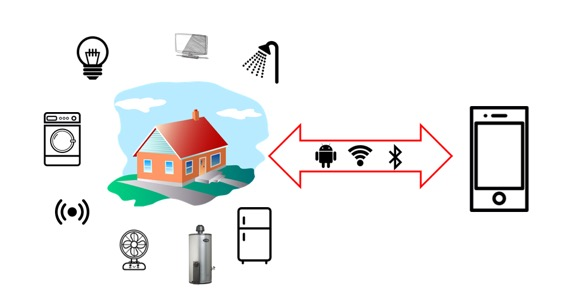
\includegraphics[scale=0.55]{Figura 1 - Domotica.jpg}
\caption[Ejemplo de sistema de domótica]{Ejemplo de sistema de domótica. \protect\footnotemark}
\label{fig:2}
\end{figure}
\footnotetext{Imagen tomada de: \url{https://intelligy.com/blog/2018/03/12/conoces-la-domotica/}}

\section{Motivación}

El uso de la tecnología para facilitar y mejorar la vida de las personas se está implementando en todo el mundo en diversos ámbitos, creando soluciones complejas e innovadoras. Los electrodomésticos e instalaciones se fabrican con posibilidades de conexión y capacidades cada vez más amplias, abarcando funcionalidades complejas que aportan al bienestar y confort de las personas.

Este proyecto nace como mejora y actualización de la tesis de grado de ingeniería, en la cual se creó un sistema similar que carecía de conectividad a Internet y utilizando tecnología que al día de hoy es obsoleta. Es por este motivo que se ha decidido hacer un proyecto académico con esta temática, pudiendo crear un sistema integral con una página web, base de datos que almacene mediciones y utilizando hardware actualizado.

\section{Estado del arte}

En el mercado actual existe una gran cantidad de sistemas de domótica, algunos privados o bajo licencias propietarias y otros con licencias de código abierto, nacionales e internacionales. Aquellas soluciones de código abierto tienen los repositorios públicos en \textit{Github} al alcance de todos para ser descargados, implementados y hasta modificados.

Del mercado internacional, podemos nombrar 2 importantes variantes:
\begin{itemize}
	\item Matter: es un estándar de conectividad de código abierto creado por la \textit{Connectivity standards alliance}. Es de los más importantes a nivel global y participan empresas como Amazon, Apple, Google, Huawei entre muchas otras. Ha crecido y tomado mucha fuerza durante el corto tiempo de vida que tiene el proyecto \citep{3}.
	\item Home assistant: software de automatización de hogares de código abierto que prioriza el control local y la privacidad. Desarrollado por una comunidad mundial de entusiastas de autodidactas y profesionales con un sentido propio \citep{4}.
\end{itemize}

En la figura \ref{fig:3} se observa un kit de Matter a la izquierda y la pantalla de la aplicación de Home Assistant a la derecha.

\begin{figure}[h]
\centering
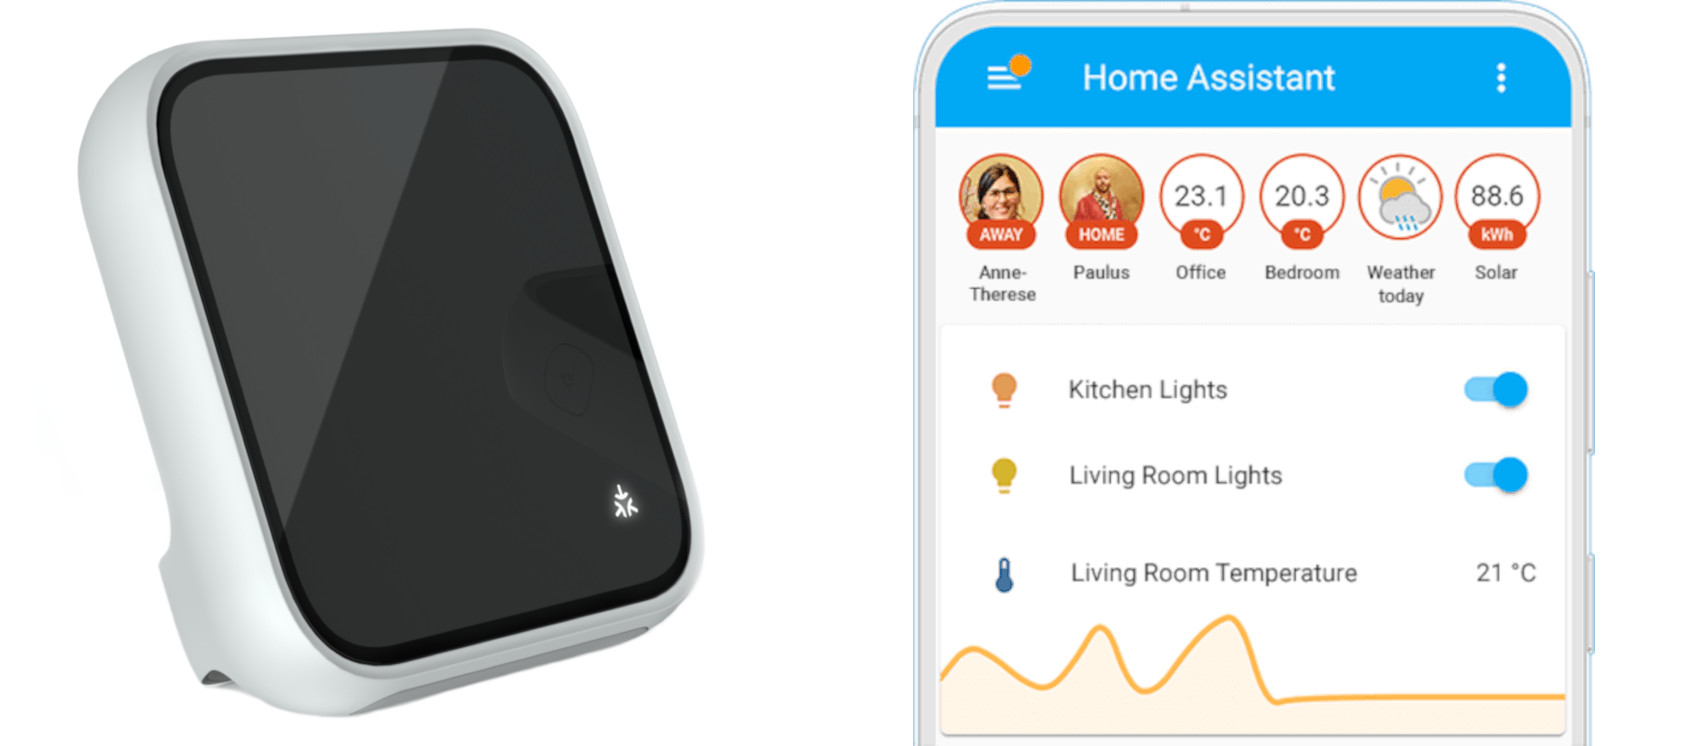
\includegraphics[scale=0.15]{Figura 2 - Soluciones.jpg}
\caption[Matter y Home Assistant]{Matter y Home Assistant. \protect\footnotemark}
\label{fig:3}
\end{figure}
\footnotetext{Imágenes tomadas de: \url{https://csa-iot.org/} y \url{https://www.home-assistant.io/}}

A nivel nacional existen empresas que se dedican al desarrollo de sistemas de domótica de forma privada:
\begin{itemize}
	\item Domotic \citep{5}.
	\item Commax \citep{6}.
	\item Reactor \citep{7}.
\end{itemize}

Todos estos sistemas utilizan distintos tipos de conexión (Zigbee o Wi-Fi), mensajes entre dispositivos (HTTP, MQTT y otros) y tipos de alojamiento de las plataformas (servidor local o en la nube).

Pocos de estos sistemas tienen la posibilidad de funcionar con mandos desde el lugar o sin conexión con el servidor, es decir, que sean independientes y controlables de forma local. Este proyecto tiene tal posibilidad, ya que la página web es una forma más de cambiar los parámetros de los nodos y está diseñado para decidir si cada terminal posee comandos o no.

En la tabla \ref{tab:empresas} pueden verse las principales características de las empresas nacionales con soluciones similares.

\begin{table}[h]
\centering
\caption[Mercado nacional]{Comparativa entre las distintas opciones}
\begin{tabular}{l c c}
\toprule
\textbf{Empresa} & \textbf{Productos} & \textbf{Compatibilidad}\\
\midrule
Domotic	& Catálogo amplio & No especifica \\
Commax	& Catálogo amplio & \textit{Smart things} y \textit{Apple Home Kit}	\\
Reactor	& 2 alternativas & \textit{Google Assistant} e \textit{IFTTT} \\
\bottomrule
\hline
\end{tabular}
\label{tab:empresas}
\end{table}

\section{Objetivos y alcance}

El objetivo de este trabajo es aplicar todos los conocimientos adquiridos en el transcurso del posgrado, en un tema de interés particular como es la domótica. En especial, el principal propósito es hacer un prototipo que dé inicio a un sistema más grande y con mayores características, con la particularidad de que en un futuro cercano se pueda llegar a analizar la opción de integrarlo con sistemas como \textit{Matter} o \textit{Home Assistant}.

En este desarrollo se incluyó:
\begin{itemize}
	\item El esquema de conexiones de las placas de ESP32 con los módulos de display, encoder, driver LED y driver de calefacción.
	\item El diseño en una placa de desarrollo del circuito del driver de corriente continua de la iluminación LED.
	\item El diseño en una placa de desarrollo del circuito del driver de corriente alterna de la calefacción.
	\item La programación de un firmware de la placa ESP32 para la comunicación y manejo de conexiones.
	\item La creación del software frontend, backend y la base de datos que almacena toda la información dentro del servidor.
	\item Las conexiones, instalación y configuración del servidor montado en una Raspberry Pi.
\end{itemize}

En la figura \ref{fig:4} se puede ver un esquema básico del sistema desarrollado.
\begin{figure}[h]
\centering
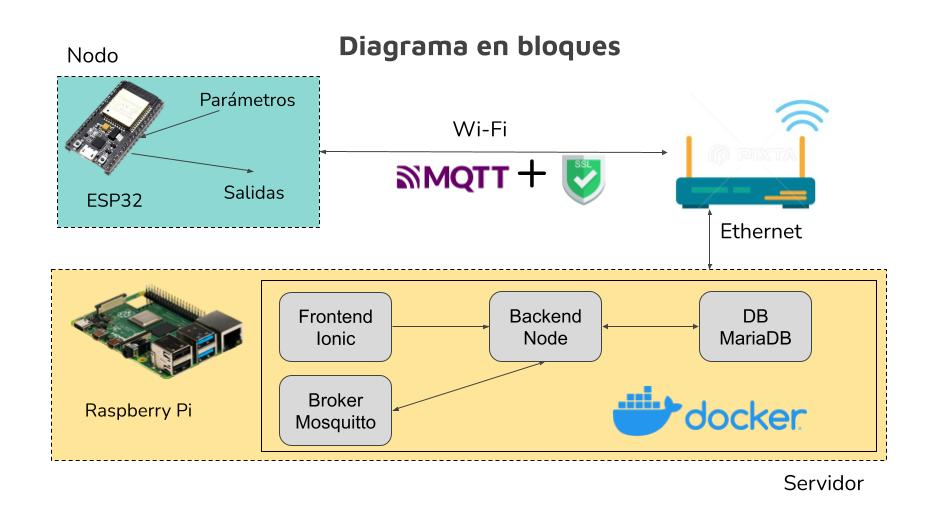
\includegraphics[scale=0.4]{Figura 3 - Diagrama en bloques.jpg}
\caption[Esquema básico]{Esquema básico del sistema desarrollado. \protect}
\label{fig:4}
\end{figure}
\chapter{Introducción específica} % Main chapter title

\label{Chapter2}

 
\chapter{Diseño e implementación}

\label{Chapter3}

En el presente capítulo se presentan los detalles del diseño y los criterios adoptados para el desarrollo del trabajo junto con los pasos seguidos para su implementación.

\section{Arquitectura del sistema}

El sistema tiene una configuración de arquitectura del tipo cliente-servidor. Está constituido por dos nodos y un servidor, los cuales están conectados a la red local y se comunican a través del protocolo MQTT. El servidor recibe los parámetros actuales de estado y cambios desde cada dispositivo, los procesa y almacena en la base de datos. También envía mensajes hacia los dispositivos para cambiar el estado de las salidas o el parámetro que se desee cambiar. Los usuarios pueden consultar y modificar el estado de los dispositivos desde un navegador web móvil o desde una computadora.

En la figura \ref{fig:9} se puede observar la arquitectura cliente-servidor del sistema implementado en el trabajo.

\begin{figure}[h]
\centering
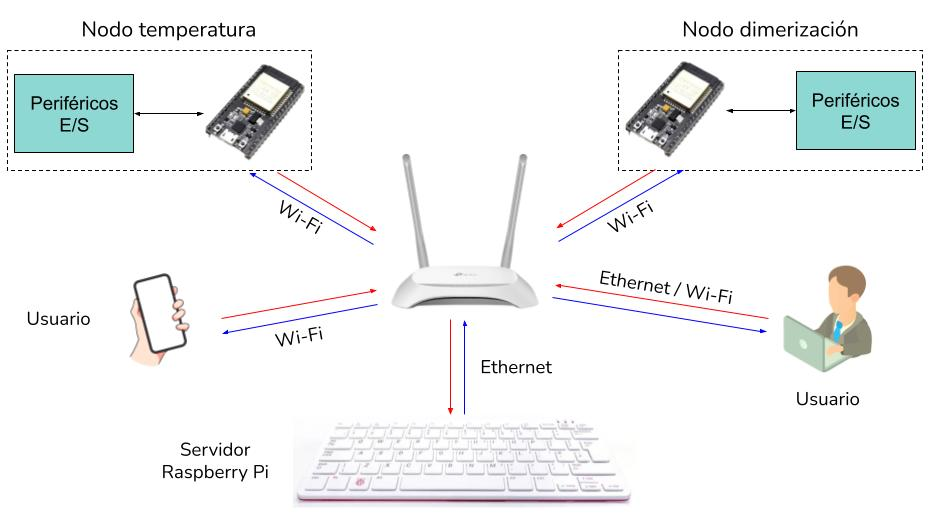
\includegraphics[scale=0.4]{Imagen 9 - cliente-servidor.jpg}
\caption[Arquitectura cliente-servidor]{Arquitectura cliente-servidor. \footnotemark}
\label{fig:9}
\end{figure}
\footnotetext{Imagen tomada de: \url{https://www.bujarra.com/raspberry-pi-servidor-vpn-con-pptp/}}

Uno de los nodos tiene como función sensar y controlar de temperatura de un recinto, y el otro controlar la iluminación. Originalmente el proyecto estaba pensado para que un solo nodo implemente estas dos funciones, pero durante el desarrollo se optó por la implementación separada. Este cambio se basó en la idea de modularizar los nodos y que sus funciones sean específicas. De esta forma es más amigable para el usuario visualizar y modificar el estado en pantalla e implementar el alta de nuevos dispositivos en el sistema.

El servidor está montado sobre una Raspberry Pi 400 con un sistema operativo Raspbian con interfaz gráfica. Este sistema operativo es la versión oficial ofrecida por la fundación Rasperry Pi y está basado en Debian versión 11 (\textit{bullseye}). En esta etapa de desarrollo se optó por una Raspberry Pi 400 por una cuestión de costos y practicidad a la hora de desarrollar y hacer las pruebas, aunque tiene un mayor volumen que los otros modelos de la familia. Al momento de ofrecer una solución definitiva está pensado que sea implementado en una placa con el formato más pequeño como cualquiera de las Raspberry Pi 4. La conexión del servidor a la red local es por cable Ethernet.

\subsection{Especificaciones técnicas del servidor}

El sistema operativo del servidor está instalado y se ejecuta desde un disco de estado sólido por USB. Este tipo de discos tienen una mayor capacidad de escrituras y lecturas que una memoria microSD, lo que resulta favorable al momento de hacer modificaciones y pruebas de ejecución de software. En la versión final del sistema todo el software estará instalado en una tarjeta microSD para que todo el conjunto sea lo más pequeño posible.

En la tabla \ref{tab:Especificaciones Raspberry Pi 400} pueden verse las especificaciones técnicas de hardware más importantes del modelo Raspberry Pi 400.

\begin{table}[h]
\centering
\caption[Raspberry Pi 400]{Especificaciones de Raspberry Pi 400.}
\begin{tabular}{l c}
\toprule
Procesador		&	Broadcom BCM2711 quad-core Cortex-A72(ARM v8) \\
				&	64-bit SoC @ 1.8GHz \\
\midrule
Memoria			&	4GB LPDDR4-3200 \\
\midrule
				&	2.4GHz and 5.0GHz 802.11b/g/n/ac wireless LAN \\
Conectividad		&	Bluetooth 5.0, BLE\\
				&   Gigabit Ethernet \\
\midrule
Alimentación		&	5V DC vía USB-C\\
\bottomrule
\hline
\end{tabular}
\label{tab:Especificaciones Raspberry Pi 400}
\end{table}

\section{Modelo de datos}

En esta sección se describen las diferentes tablas dentro de la base de datos de tipo relacional MariaDB. Con el objetivo de mostrar una representación visual fácil de comprender se muestran las imágenes representadas en la página phpMyadmin. Las tablas que forman dicha base son:

\begin{itemize}
	\item Dispositivos.
	\item Usuarios.
	\item Mediciones.
\end{itemize}

Debe tenerse en cuenta que todo el contenido que se ejecuta del lado del servidor se encuentra dentro de un contenedor Docker. Dicho contenido corresponde a las imágenes de los servicios de Ionic, MariaDB, phpMyAdmin, backend con Node y mosquitto. En la figura \ref{fig:10} se observa el contenido del archivo \textit{docker-compose.yml} pertinente a la configuración de los servicios de MariaDB y phpMyAdmin.

\begin{figure}[h]
\centering
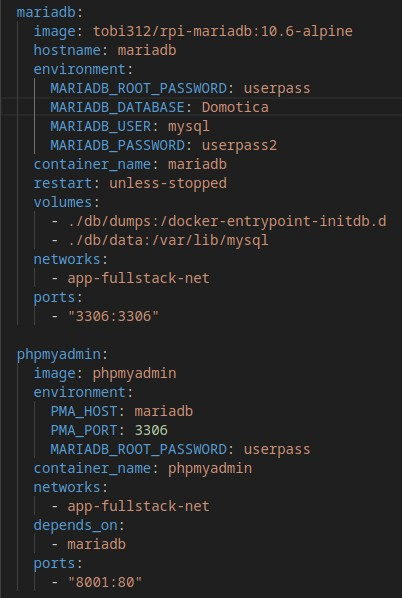
\includegraphics[scale=0.6]{Imagen 10 - Docker base datos.jpg}
\caption[Docker base datos]{Configuración de Docker de la base de datos. \footnotemark}
\label{fig:10}
\end{figure}

\subsection{Tabla Dispositivos}

Esta tabla contiene los datos de los dispositivos dados de alta en el sistema. Dichos datos son el ID del dispositivo, el nombre, la ubicación, la dirección MAC, el tipo, el valor de la alarma y el estado de la alarma (0 para desactivada y 1 para activada).

En la figura \ref{fig:11} puede verse la tabla cargada con 2 dispositivos funcionando.

\begin{figure}[h]
\centering
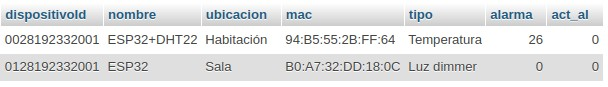
\includegraphics[scale=0.6]{Imagen 11 - Tabla dispositivos.jpg}
\caption[Tabla dispositivos]{Tabla de dispositivos. \footnotemark}
\label{fig:11}
\end{figure}

El ID del dispositivo es un número brindado por el fabricante del dispositivo que consta de 13 números y está formado por: los primeros 2 dígitos que corresponden al tipo de dispositivo (el sistema está pensado para cubrir hasta un total de 100 tipos de dispositivos, aunque en esta etapa de prototipo sólo se hayan desarrollado 2); 4 dígitos de seguridad fijos que en este caso son "2819" y sirven para corroboración y como seguridad; y los últimos 5 dígitos corresponden al número de serie del equipo (2 para el año, 2 para la semana y 3 para el número de fabricación del equipo en esa semana, en ese orden). Como puede observarse, el sistema está pensado para que en un futuro sea parte de una producción en serie.

Tanto el nombre como la ubicación son campos alfanuméricos elegidos por el usuario para describir al dispositivo. La dirección MAC es enviada por el dispositivo la primera vez que se conecta al sistema y no se completa por el usuario. El tipo corresponde al tipo de sensor y para esta etapa del desarrollo puede ser "Temperatura" o "Luz dimmer".

El valor de la alarma es un campo numérico y sólo tiene efecto para dispositivos del tipo de temperatura. Se enviará una notificación por mail cada vez que el valor enviado por el dispositivo sea mayor o igual al seteado en este campo, siempre que dicha alarma esté activada en el campo.

\subsection{Tabla Usuarios}

La tabla de usuarios contiene todos los datos relacionados a aquellas personas que vayan a utilizar el sistema. En esta etapa está implementado con 3 usuarios, ya que al ser de tipo hogareño resultaría difícil que más de 3 personar dentro de una misma casa se registren. Pero con pocos cambios el sistema podría ser escalable a la cantidad de usuarios que se desee, generando una página de alta de usuarios.

Los valores almacenados en esta tabla son el ID de usuario (de 1 a 3), el nombre de usuario, la clave, el nombre de la persona y su apellido, su e-mail y un campo de tipo booleano que se modificará cuando se haya actualizado por primera vez. Cabe aclarar que cada vez que se ingrese al sistema con un usuario que no haya actualizado sus datos, se mostrará en pantalla un aviso para que este actualice sus datos.

En la figura \ref{fig:12} puede verse la tabla cargada con los 3 usuarios de los cuales hay 2 actualizados y el tercero tiene los valores por defecto.

\begin{figure}[h]
\centering
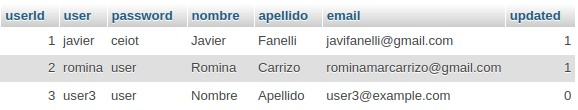
\includegraphics[scale=0.6]{Imagen 12 - Tabla usuarios.jpg}
\caption[Tabla usuarios]{Tabla de usuarios. \footnotemark}
\label{fig:12}
\end{figure}

\subsection{Tabla Mediciones}

La tabla de mediciones contiene todos los datos referentes a las mediciones realizadas por los dispositivos y los datos de modo seleccionado. Los dispositivos reportan cada 5 minutos estos datos y se almacenan en esta tabla.

Los datos almacenados en esta tabla son: el ID de la medición (un valor autoincremental), el ID del dispositivo, el tipo de dispositivo, la fecha y hora de la medición, el valor de la medición, el modo de funcionamiento (manual o automático), el valor de la salida (si es de tipo temperatura es 0 o 100 y corresponde a encendido o apagado, y si es de tipo luz dimmer va de 0 a 100 con saltos de 10), y la hora y minutos de encendido y apagado para el modo automático.

En la figura \ref{fig:13} pueden verse algunas de las mediciones dentro de la correspondiente tabla, ordenadas por ID. Cabe aclarar que sólo se ven algunas ya que los dispositivos se encuentran reportando y llenando de datos la base.

\begin{figure}[h]
\centering
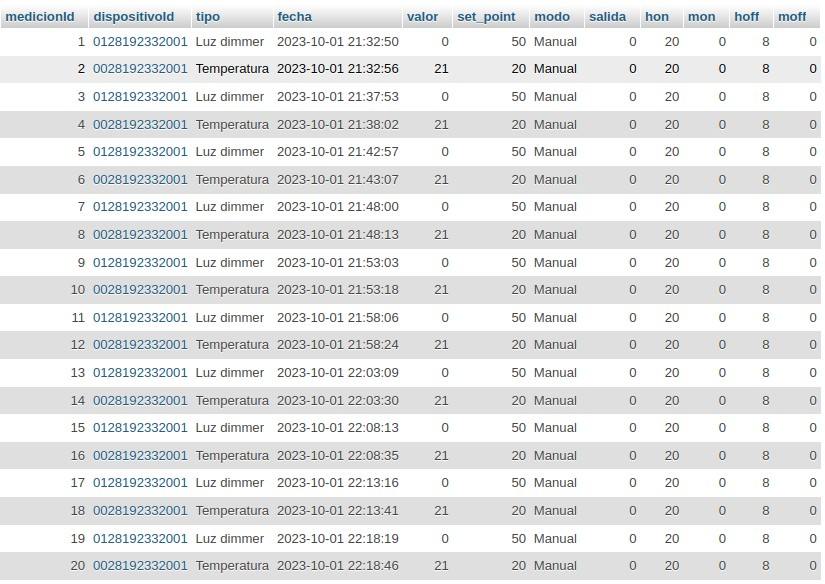
\includegraphics[scale=0.6]{Imagen 13 - Tabla mediciones.jpg}
\caption[Tabla mediciones]{Tabla de mediciones. \footnotemark}
\label{fig:13}
\end{figure}

\section{Desarrollo del frontend}

El frontend del presente trabajo fue desarrollado en el lenguaje TypeScript con Angular como \textit{framework} integrado con Ionic. El prototipo de aplicación está diseñado para acceder desde un navegador web tanto desde una computadora como un móvil, pero se optó por usar Ionic para un posterior desarrollo de una aplicación para sistemas operativos móviles. Es por esto que en esta instancia puede referirse a la aplicación web como una SPA y no como una PWA.

En la figura \ref{fig:14} se puede observar el fragmento de código correspondiente a la configuración de Ionic dentro del archivo \textit{docker-compose.yml}.

\begin{figure}[h]
\centering
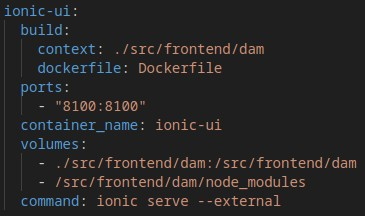
\includegraphics[scale=0.6]{Imagen 14 - Docker ionic.jpg}
\caption[Configuración Ionic]{Configuración de Docker de Ionic. \footnotemark}
\label{fig:14}
\end{figure}

La estructura de archivos de cada página esta diseñada de la misma forma como se muestra en la imagen \ref{fig:15}. Allí se pueden ver como ejemplo los archivos que componen la página \textit{home}.

\begin{figure}[h]
\centering
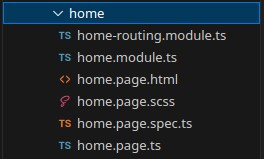
\includegraphics[scale=0.6]{Imagen 15 - Estructura.jpg}
\caption[Estructura página]{Estructura de archivos de página. \footnotemark}
\label{fig:15}
\end{figure}

Además se utilizaron interfaces para definir las estructuras de datos de los dispositivos, las mediciones y los usuarios, y servicios para el proceso de autenticación y de consultas HTTP al backend, que serán explicadas posteriormente.

El servicio de autenticación consta de el ingreso de un usuario y contraseña en la página de \textit{login} que se comparan con los que están almacenados en la base de datos. Si dichos valores ingresados corresponden con alguno de los existentes, se genera un \textit{token} desde el backend que se almacena en el dispositivo que está haciendo la consulta. Esto permite que se puedan acceder a las demás páginas de la aplicación.

En el código \ref{lst:Autenticación de rutas} puede verse el fragmento de la autenticación del archivo \textit{auth.guard.ts}

\definecolor{dkgreen}{rgb}{0,0.6,0}
\definecolor{gray}{rgb}{0.5,0.5,0.5}
\definecolor{mauve}{rgb}{0.58,0,0.82}

\lstset{frame=tb,
  language=Java,
  aboveskip=3mm,
  belowskip=3mm,
  captionpos=b,
  showstringspaces=false,
  columns=flexible,
  basicstyle={\small\ttfamily},
  numbers=left,
  numberstyle=\tiny\color{gray},
  keywordstyle=\color{blue},
  commentstyle=\color{dkgreen},
  stringstyle=\color{mauve},
  breaklines=true,
  breakatwhitespace=true,
  tabsize=3,
}

\begin{lstlisting}[caption={Autenticación de rutas}, label={lst:Autenticación de rutas}]
export class AuthGuard {
  constructor(private _loginService: LoginService, private _router: Router) {}
  canActivate(
    route: ActivatedRouteSnapshot,
    state: RouterStateSnapshot): Observable<boolean | UrlTree> | Promise<boolean | UrlTree> | boolean | UrlTree {
    if (!this._loginService.logIn) {
      this._router.navigate(['/login'])
      return false
    }
    return true;
  }
}
\end{lstlisting}

El \textit{route guard} es una característica del Angular Router que permite ejecutar algún tipo de lógica cuando se solicita una ruta, y basado en esa lógica, se permite o denega el acceso al usuario a esa ruta. Comúnmente es utilizado para verificar si un usuario está logueado o no en el sistema para verificar si tiene autorización para acceder a esa URL.

El \textit{route guard} se puede agregar implementando la interfaz \textit{CanActivate} disponible en \textit{@angular/router} y allí implementar el método \textit{canActivate()} que contendrá la lógica para denegar o permitir el acceso a la ruta.\citep{22}

\subsection{Rutas y páginas más importantes}

Las rutas disponibles en la aplicación se describen en la tabla \ref{tab:rutas}. A través de ellas se navega dentro de la aplicación y se accede a las distintas pantallas. Estas rutas se encuentran definidas en el archivo \textit{app-routing.module.ts} donde además se hace referencia al módulo de la aplicación que debe abrirse al acceder a cada una de las rutas listadas.

\begin{table}[h]
\centering
\caption[Rutas]{Rutas de la aplicación}
\begin{tabular}{l l}
\toprule
\textbf{Ruta} 			& \textbf{Descripción}\\
\midrule
/login					& Pantalla de inicio de sesión\\
/home					& Pantalla principal con funciones y listado de dispositivos\\
/usuario/:userId			& Pantalla de edición de datos de usuario\\
/ayuda					& Pantalla de manual de usuario\\
/dispositivos/:id		& Pantalla de visualización de estado del dispositivo\\
/medicion/:id			& Pantalla de visualización de las mediciones del\\
/grafico/:id				& Pantalla de visualización del gráfico de las mediciones\\
/config/:id				& Pantalla de configuración del dispositivo\\
/modificar/:id			& Pantalla de edición de datos de un dispositivo existente\\
/agregar					& Pantalla para agregar un dispositivo nuevo\\
\bottomrule
\hline
\end{tabular}
\label{tab:rutas}
\end{table}

En los casos en los que se encuentra el campo \textit{:id}, este valor se completa con el valor de identificador del elemento en cuestión. En el caso de los usuarios, cada uno de ellos tiene un identificador, lo mismo que para los dispositivos. Para las rutas \textit{medicion}, \textit{grafico}, \textit{config} y \textit{modificar} el \textit{:id} al que se hace referencia es el del dispositivo al que se quiere leer o modificar.

\subsubsection{Pantalla de \textit{login}}

En la figura \ref{fig:16} se muestra la página de inicio de sesión en la aplicación.

\begin{figure}[h]
\centering
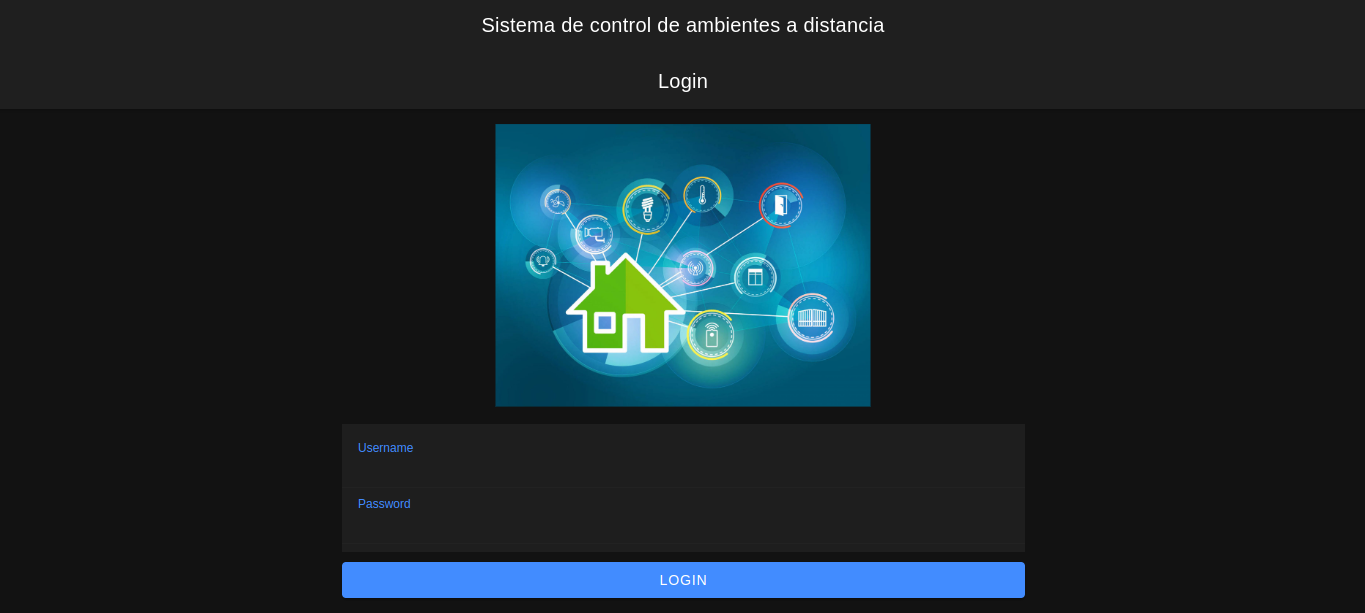
\includegraphics[scale=0.38]{Imagen 16 - Login.png}
\caption[Pantalla login]{Pantalla de \textit{login}. \footnotemark}
\label{fig:16}
\end{figure}

El sistema trae la posibilidad de configurar 3 usuarios distintos para que utilicen, visualicen y configuren la aplicación. Todos poseen el mismo rol y pueden configurar cualquier campo que corresponda a dicho usuario ingresando en la opción Usuario dentro de la pantalla principal.

\subsubsection{Pantalla principal \textit{home}}

En la figura \ref{fig:17} puede verse la pantalla principal de la aplicación. En la parte superior se encuentran los botones principales de la aplicación tales como el de configuración del usuario actual, cerrar sesión y la página de ayuda o manual de usuario. En la parte inferior se encuentra el listado de dispositivos implementado con \textit{ion-cards} los cuales permiten ver el estado de cada dispositivo, modificar los datos y alarma del dispositivo y eliminarlo de la lista. Hay que tener en cuenta que al borrar un dispositivo del sistema se borran también todas las mediciones y documentos asociados a él dentro de la base de datos.

\begin{figure}[h]
\centering
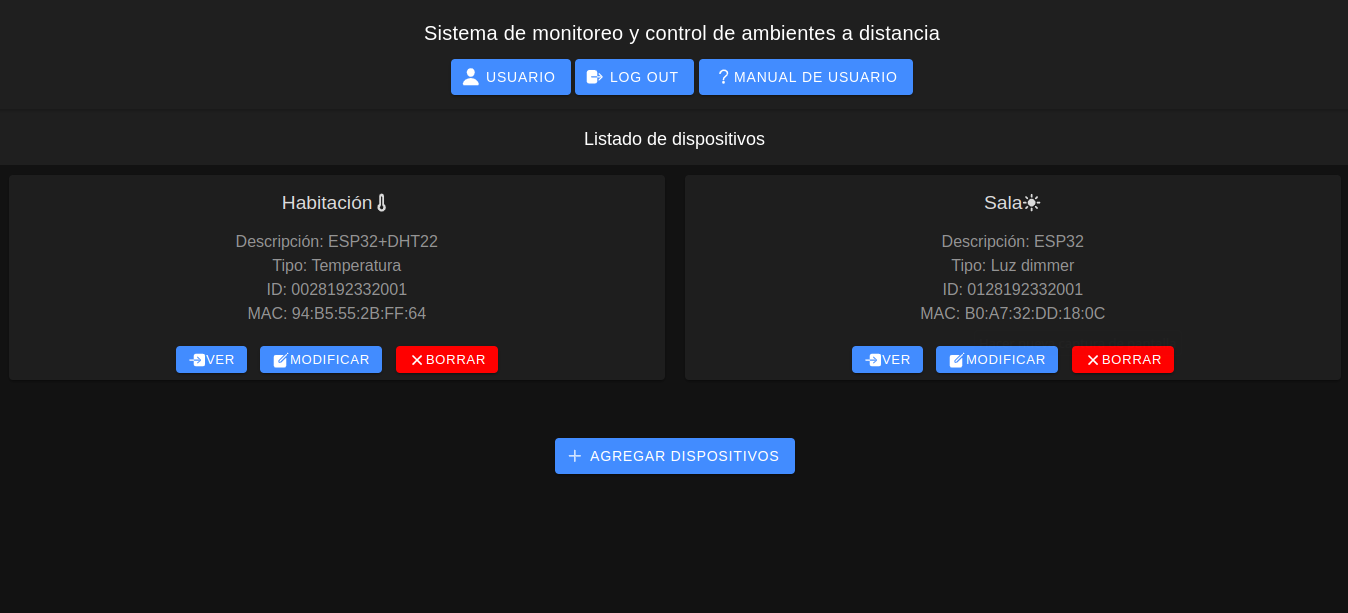
\includegraphics[scale=0.38]{Imagen 17 - Home.png}
\caption[Pantalla home]{Pantalla de \textit{home}. \footnotemark}
\label{fig:17}
\end{figure}

Por último en la parte inferior de la pantalla principal se encuentra el botón para agregar un dispositivo nuevo. Dicho botón dirige a la página de creación de un dispositivo nuevo.

\subsubsection{Pantalla de creación de dispositivo nuevo}

En la pantalla que se muestra en la figura \ref{fig:18} se deben cargar los datos de un dispositivo nuevo. Esto es importante ya que aquí se dan de alta los dispositivos nuevos que se incorporar al sistema.

\begin{figure}[h]
\centering
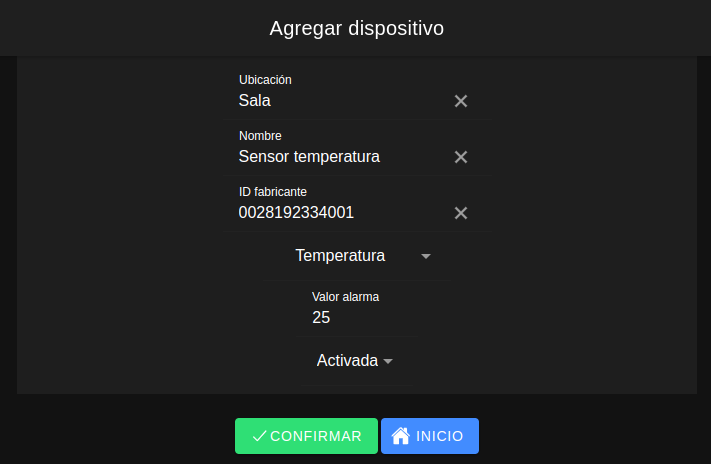
\includegraphics[scale=0.45]{Imagen 18 - Agregar.png}
\caption[Pantalla home]{Pantalla de creación de dispositivo nuevo. \footnotemark}
\label{fig:18}
\end{figure}

Aquí deben colocarse los datos de ubicación del nodo, el nombre con el que se desea identificarlo, el ID de fabricante, el tipo, y los valores de la alarma en caso de que se trate de un nodo de temperatura. El estado de la alarma puede configurarse pro primera vez en esta sección, pero puede modificarse cuando se desee. Se debe tener en cuenta que al momento existen 2 tipos de dispositivos: temperatura y luz dimmer. Solo se encuentra habilitada la alarma para los nodos del tipo de temperatura ya que no tiene sentido colocar una alarma a un nodo que no realiza mediciones ni controla parámetros críticos.

El ID del fabricante es un número de 13 dígitos compuesto de la siguiente forma: los 2 primeros identifican el tipo de dispositivo; los 4 que le siguen son obligatoriamente los números "2819", y se colocan como número de identificación del sistema y como seguridad; los 2 dígitos que le siguen son el año de fabricación del dispositivo; los 2 que le siguen son la semana de fabricación; y por último los 3 dígitos que restan son el número de fabricación en esa semana, es decir que comienza en el "000" y termina en "999". Este número resultante será entregado por el fabricante y será único para cada dispositivo.

Desde el frontend se verifica que se ingrese el código de seguridad dentro del ID del fabricante en el fragmento de código \ref{lst:Verificación de ID}:

\begin{lstlisting}[caption={Verificación de ID}, label={lst:Verificación de ID}]
verificarID(dispositivoId: string): boolean {
    const posicion = 2;
    return dispositivoId.charAt(posicion) === '2' &&
      dispositivoId.charAt(posicion + 1) === '8' &&
      dispositivoId.charAt(posicion + 2) === '1' &&
      dispositivoId.charAt(posicion + 3) === '9';
  }
\end{lstlisting}

Una vez que el dispositivo nuevo esté dado de alta, al encenderlo se va a conectar a la red y va a registrar automáticamente la dirección MAC dejándola guardada en la tabla de dispositivos.

\subsubsection{Pantalla de configuración de modo}

En esta sección se va a configurar el modo de trabajo y todos los parámetros asociados.

\begin{figure}[h]
\centering
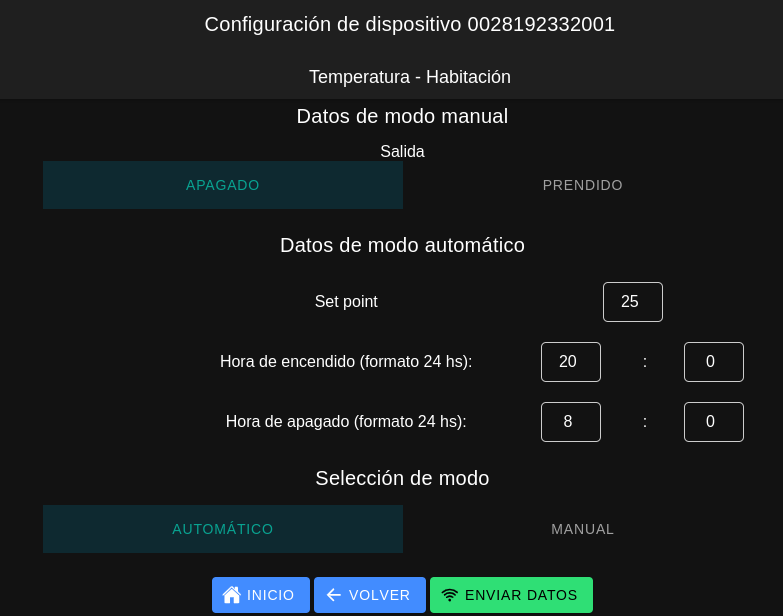
\includegraphics[scale=0.45]{Imagen 19 - Enviar datos.png}
\caption[Pantalla de configuración de modo]{Pantalla de configuración de modo. \footnotemark}
\label{fig:19}
\end{figure}

\section{Desarrollo del backend}



\section{Nodos, sensores y actuadores}

Los nodos están compuestos por el módulo central y los periféricos de entrada y salida. En el desarrollo del prototipo se utilizaron 2 versiones de módulo central, una que cuenta con un microcontrolador ESP32 para el nodo que controla temperatura y otra que cuenta con un ESP32 para el nodo que controla la iluminación dimerizable. En la tabla \ref{tab:esp32} pueden verse las características más importantes de ambos modelos de microcontroladores.

\begin{table}[h]
\centering
\caption[Módulos ESP32]{Especificaciones técnicas de los módulos ESP32.}
\begin{tabular}{l c c}
\toprule
\textbf{Característica} & \textbf{ESP32} & \textbf{ESP32C3}\\
\midrule
Núcleo			& Xtensa® dual-core 32-bit LX6 	& 32-bit single-core RISC-V \\
				& @240 MHz						& @160 MHz \\
Flash			& 0 MB, 2 MB o 4MB				& 0 MB o 4 MB \\
				& (dependiendo la versión)		& (dependiendo la versión) \\
Protocolo Wi-Fi	& 802.11 b/g/n, 2.4 GHz			& 802.11 b/g/n, 2.4 GHz \\
\bottomrule
\hline
\end{tabular}
\label{tab:esp32}
\end{table}

A continuación se listan periféricos utilizados como sensores y actuadores con sus principales características:
\begin{itemize}
	\item DHT22: sensor de temperatura y humedad relativa ambiente.
	\begin{itemize}
		\item Rango de temperatura: -40 a 80 grados Celsius.
		\item Resolución: 0,1 grado Celsius.
		\item Comunicación: serie, bus de 1 hilo, 40 bits por trama.
	\end{itemize}
	\item KY-040: encoder rotativo con interruptor cuya función es cambiar los parámetros desde el nodo. 20 pulsos por vuelta.
	\item SSD1306: display OLED 1,2 pulgadas.
	\begin{itemize}
		\item Resolución: 128x64 píxeles.
		\item Interfaz: I2C.
	\end{itemize}
	\item Control de potencia para 220 V: módulo con aislación y salida de triac para control de la calefacción. Se puede utilizar también para cualquier tipo de carga de 220 V 50 Hz.
	\begin{itemize}
		\item Tipo: encendido - apagado (on - off).
		\item Carga máxima: 8 A.
		\item Tipo de aislación: optoacoplador.
		\item Tensión máxima de aislación: 7500 V AC pico, 1 segundo de duración.
	\end{itemize}
	\item Control de intensidad de luz: módulo de control para iluminación LED de corriente continua implementado con modulación por ancho de pulso (PWM). También se puede utilizar como módulo de encendido y apagado para cualquier tipo de cargas de corriente continua.
	\begin{itemize}
		\item Tipo: PWM y encendido - apagado (on - off).
		\item Carga máxima: 800 mA CC.
		\item Tensión de alimentación: 5 a 24 V CC.
	\end{itemize}
\end{itemize}

En la imagen 2.4 puede observarse el diagrama en bloques del nodo de temperatura y control de calefacción. Los periféricos de entrada son el encoder y el sensor de temperatura y los de salida son el display que muestra la información y la salida de potencia.

\begin{figure}[h]
\centering
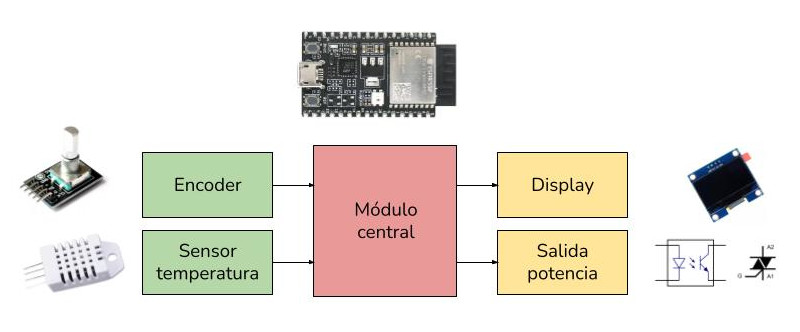
\includegraphics[scale=2]{Imagen 7 - Nodo temperatura.jpg}
\caption[Nodo de temperatura]{Diagrama en bloques del nodo de temperatura.}
\label{fig:4}
\end{figure}

En la figura 2.5 puede verse el diagrama en bloques del nodo de dimerización de la luminaria de corriente continua. En este caso, a diferencia del modelo descripto antes, posee un solo periférico de entrada y el de salida controla una salida de corriente continua de 5 a 24 V. En el caso del proyecto se utilizó una luminaria de 5 V y un consumo de 200 mA.

\begin{figure}[h]
\centering
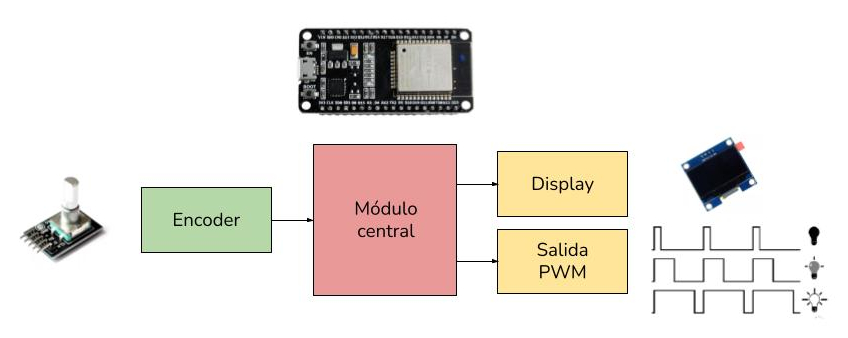
\includegraphics[scale=2]{Imagen 8 - Nodo dimmer.jpg}
\caption[Nodo dimer]{Diagrama en bloques del nodo de dimerización.}
\label{fig:4}
\end{figure}

\section{Comunicación del sistema}
\chapter{Ensayos y resultados}

\label{Chapter4}

En este capítulo se detallan los ensayos realizados al sistema completo y los resultados obtenidos durante las pruebas de funcionamiento.

\section{Banco de pruebas}

El sistema consta físicamente de dos tipos de componentes: nodos y servidor. El servidor incluye tanto la aplicación en el frontend y el backend con sus respectivos módulos. Además, el sistema posee dos tipos de nodos: uno para el control de calefacción y otro para el control de iluminación.

Para ensayar el nodo de temperatura, se utilizaron los materiales que lo conforman que se muestran en la figura \ref{fig:31}.

\begin{figure}[h]
\centering
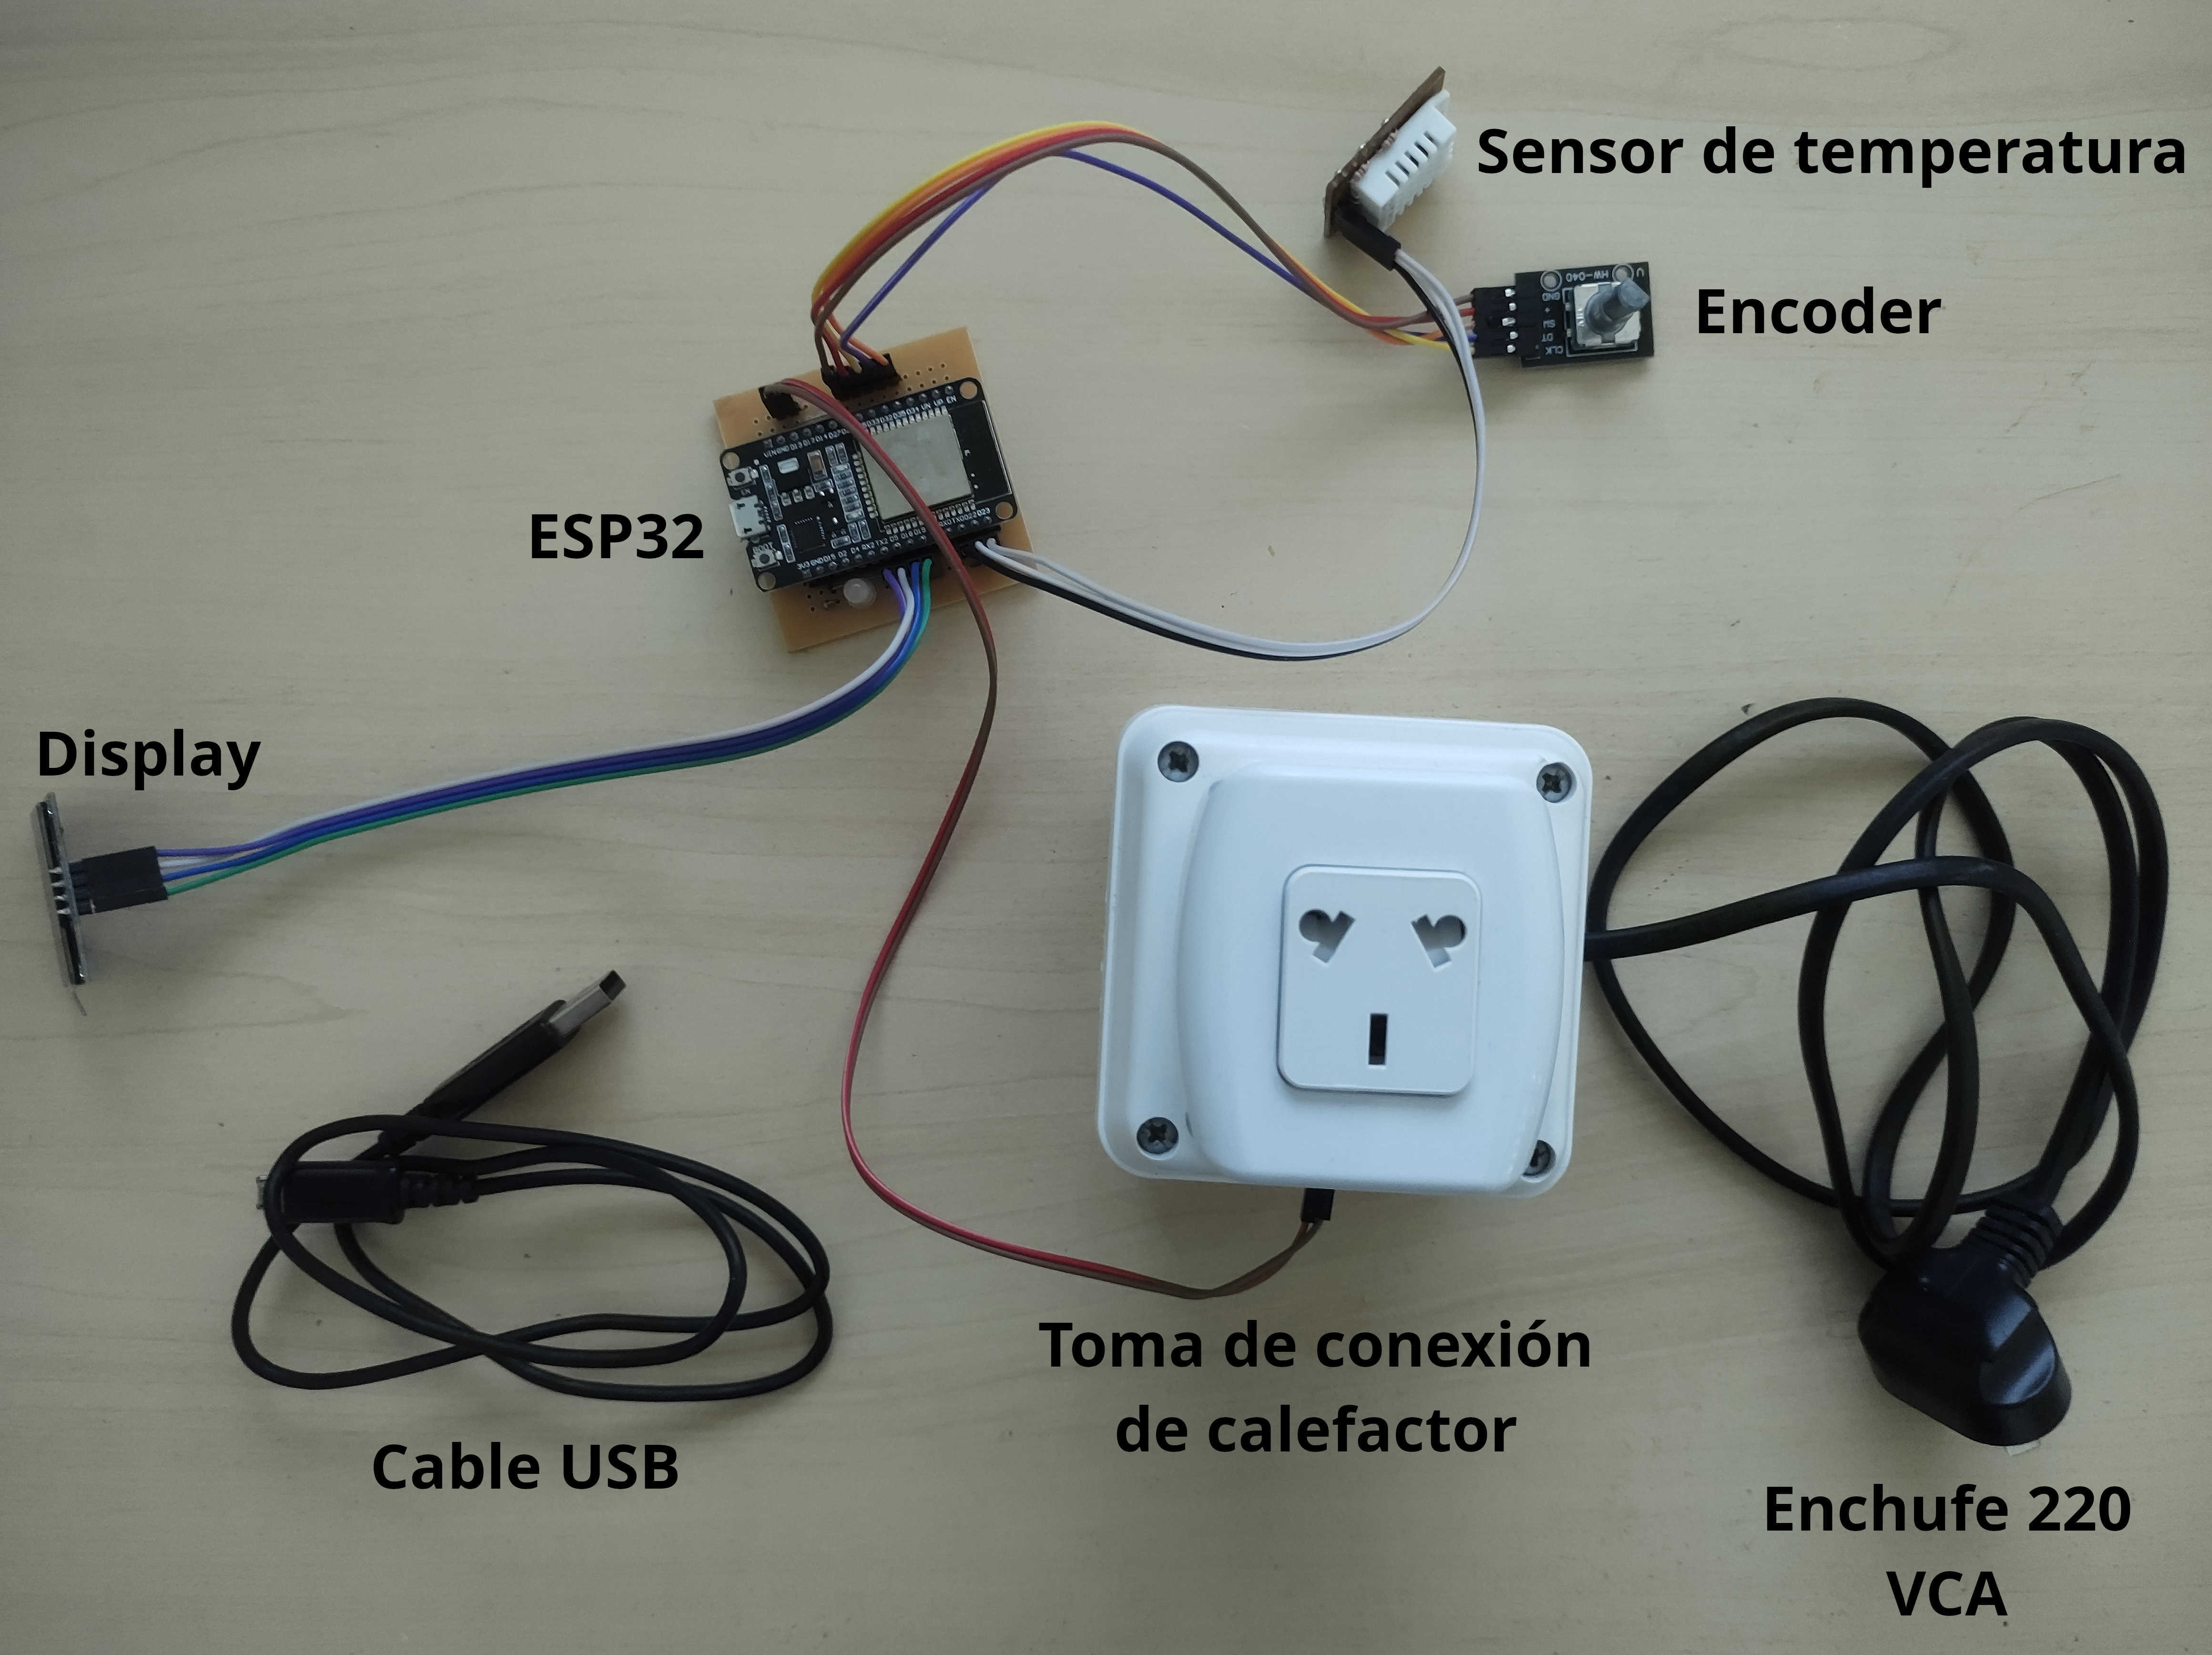
\includegraphics[scale=0.25]{Figura 31 - Nodo temperatura.jpg}
\caption[Componentes del nodo de temperatura]{Componentes del nodo de temperatura.}
\label{fig:31}
\end{figure}

En la figura \ref{fig:31}, se puede observar la placa ESP32 montada sobre la placa de conexiones, el display, el encoder, el sensor de temperatura y una caja estanca con una conexión de toma corriente para conectar la estufa a encender. Además, esta caja incluye un cable para conectarse a una fuente de alimentación de 220 VCA, que actúa como un interruptor. Cabe aclarar que en modo automático, el control de temperatura opera con una histéresis de 1 grado. Esto significa que al configurar una temperatura específica, el control apagará la salida cuando la temperatura supere en 1 grado al set-point y la encenderá cuando esté 1 grado por debajo de este valor.

Para ensayar el nodo de dimerización, se utilizaron los materiales que lo conforman que se muestran en la figura \ref{fig:32}.

\begin{figure}[h]
\centering
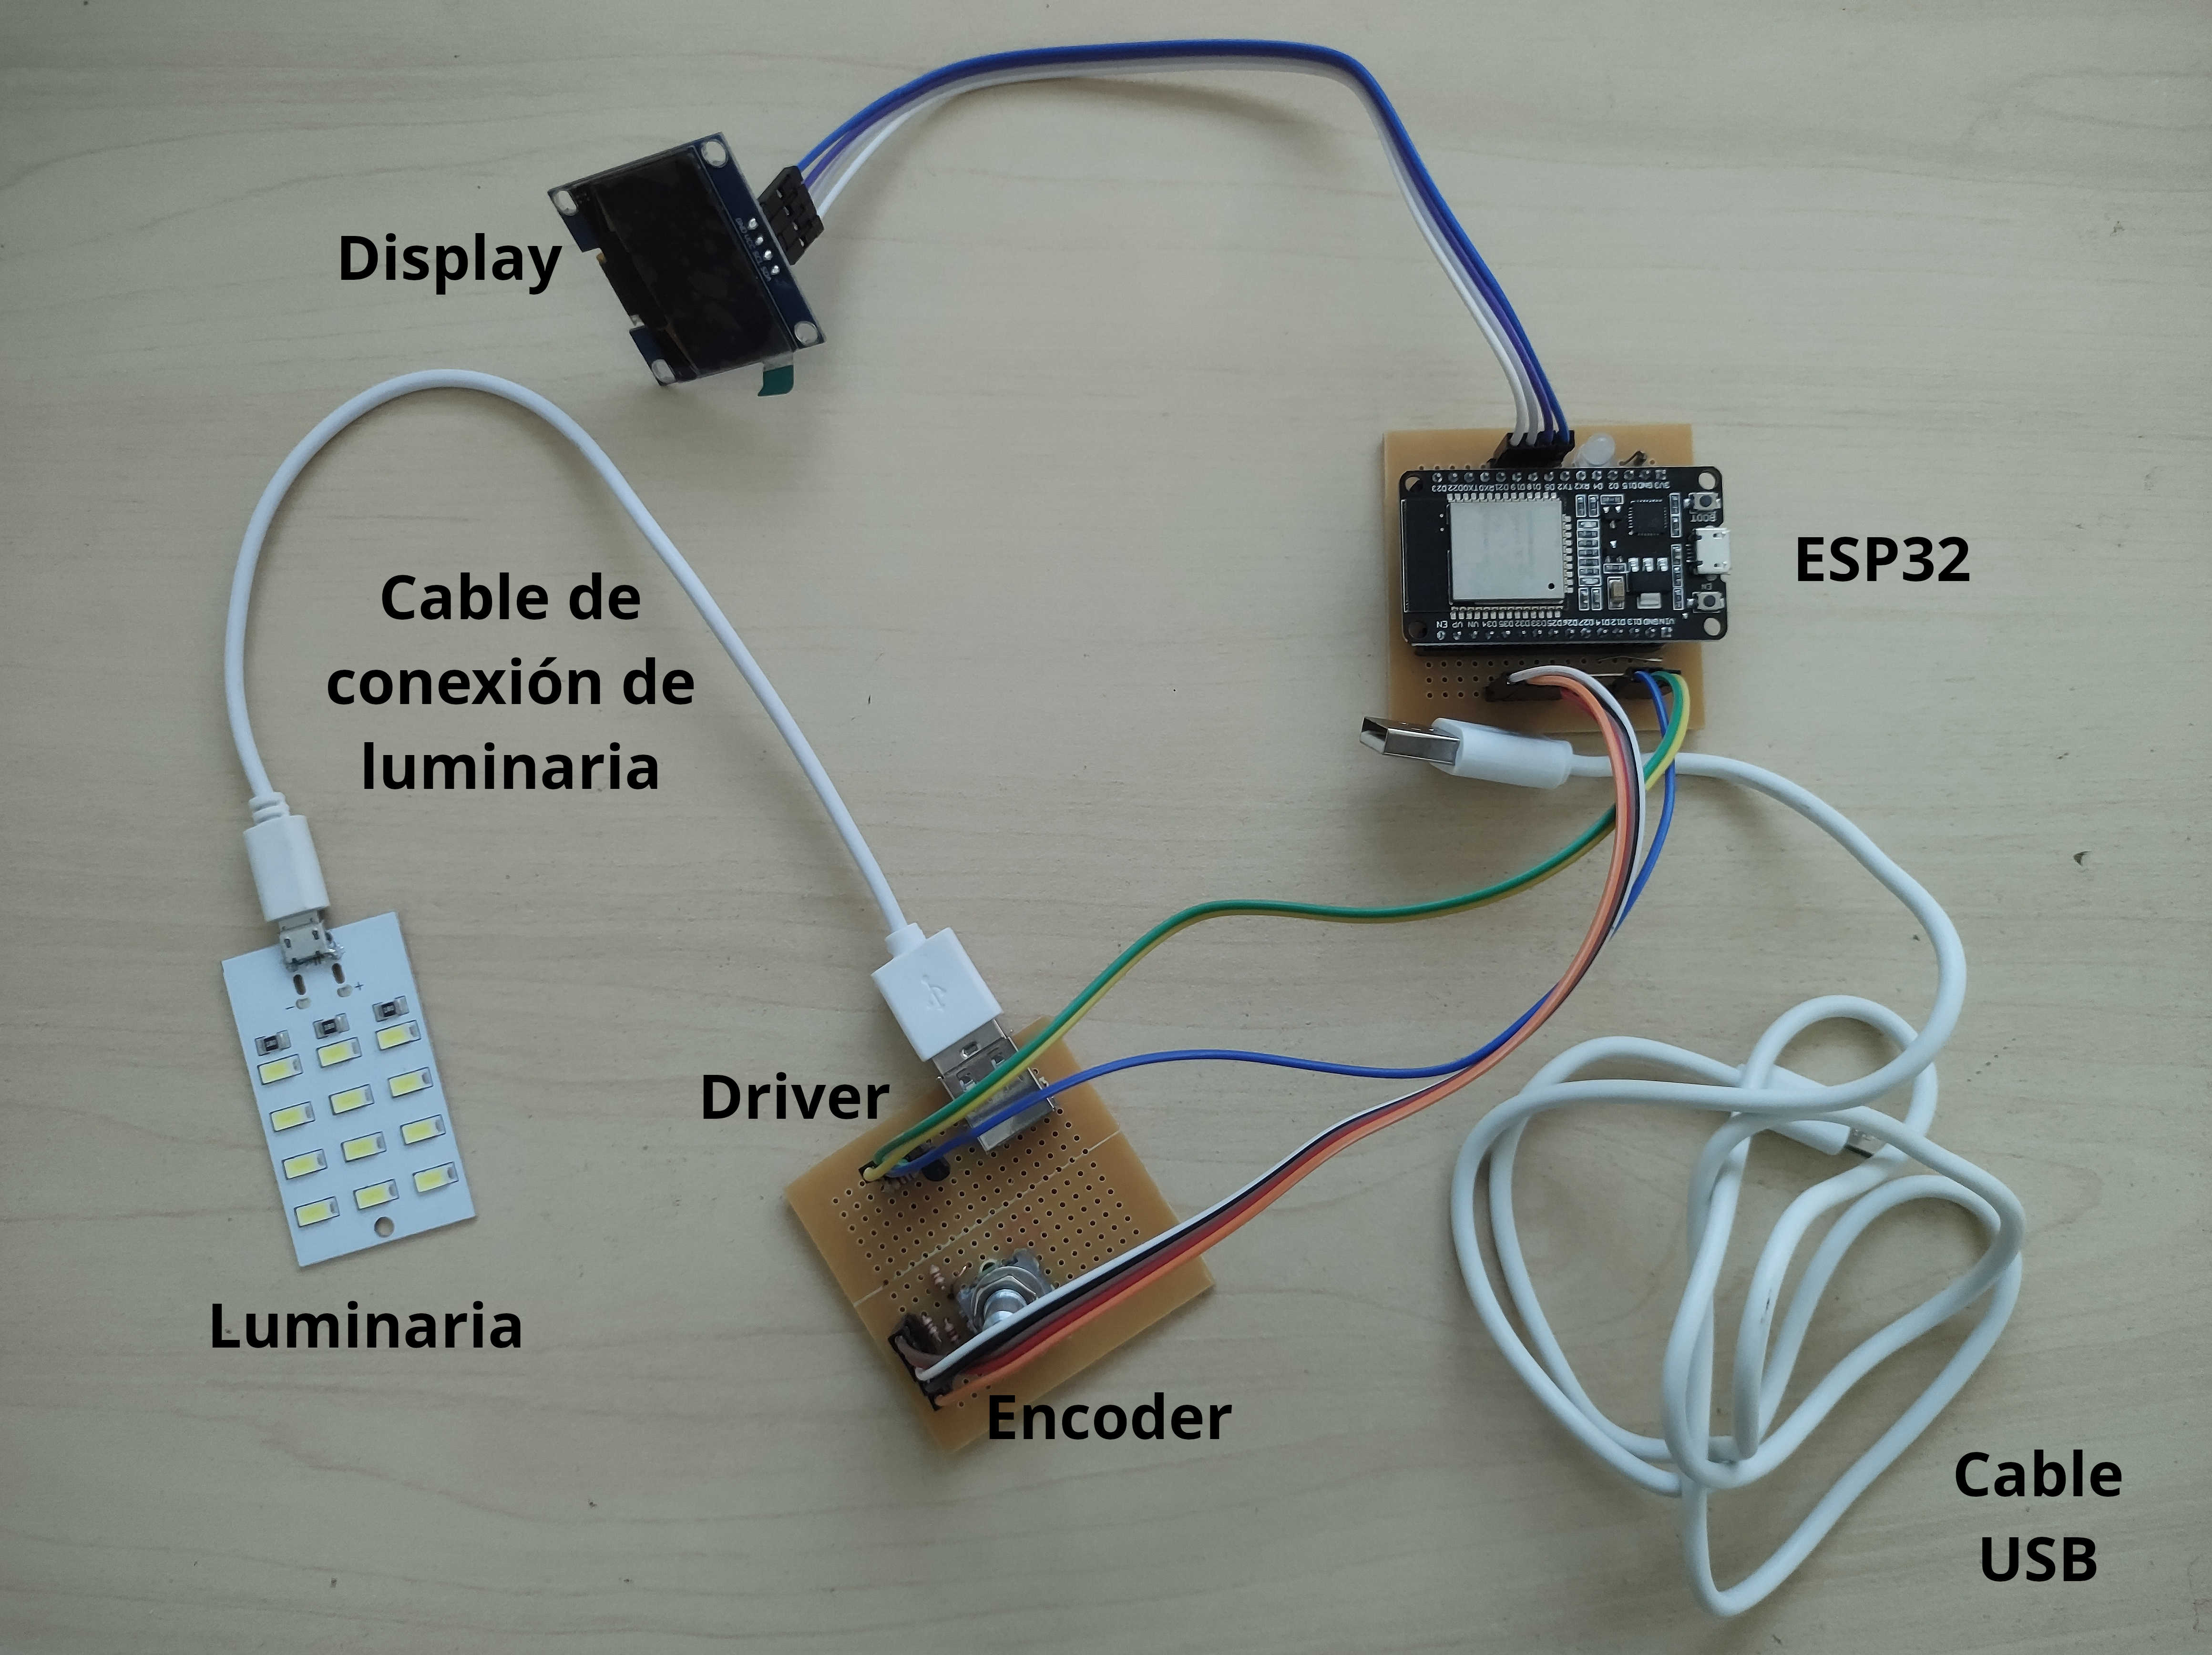
\includegraphics[scale=0.25]{Figura 32 - Nodo dimmer.jpg}
\caption[Componentes del nodo de dimerización]{Componentes del nodo de dimerización.}
\label{fig:32}
\end{figure}

En la figura  \ref{fig:32} se puede observar la placa ESP32 montada sobre la placa de conexiones, el display, el encoder, el \textit{driver} de iluminación y la placa de LEDs de 5 VCC. El control posee un conector USB por lo que puede conectarse cualquier lámpara que funcione en este caso con 5 VCC y posea este conector.

En la figura \ref{fig:33} pueden verse los componentes que forman parte del servidor.

\begin{figure}[h]
\centering
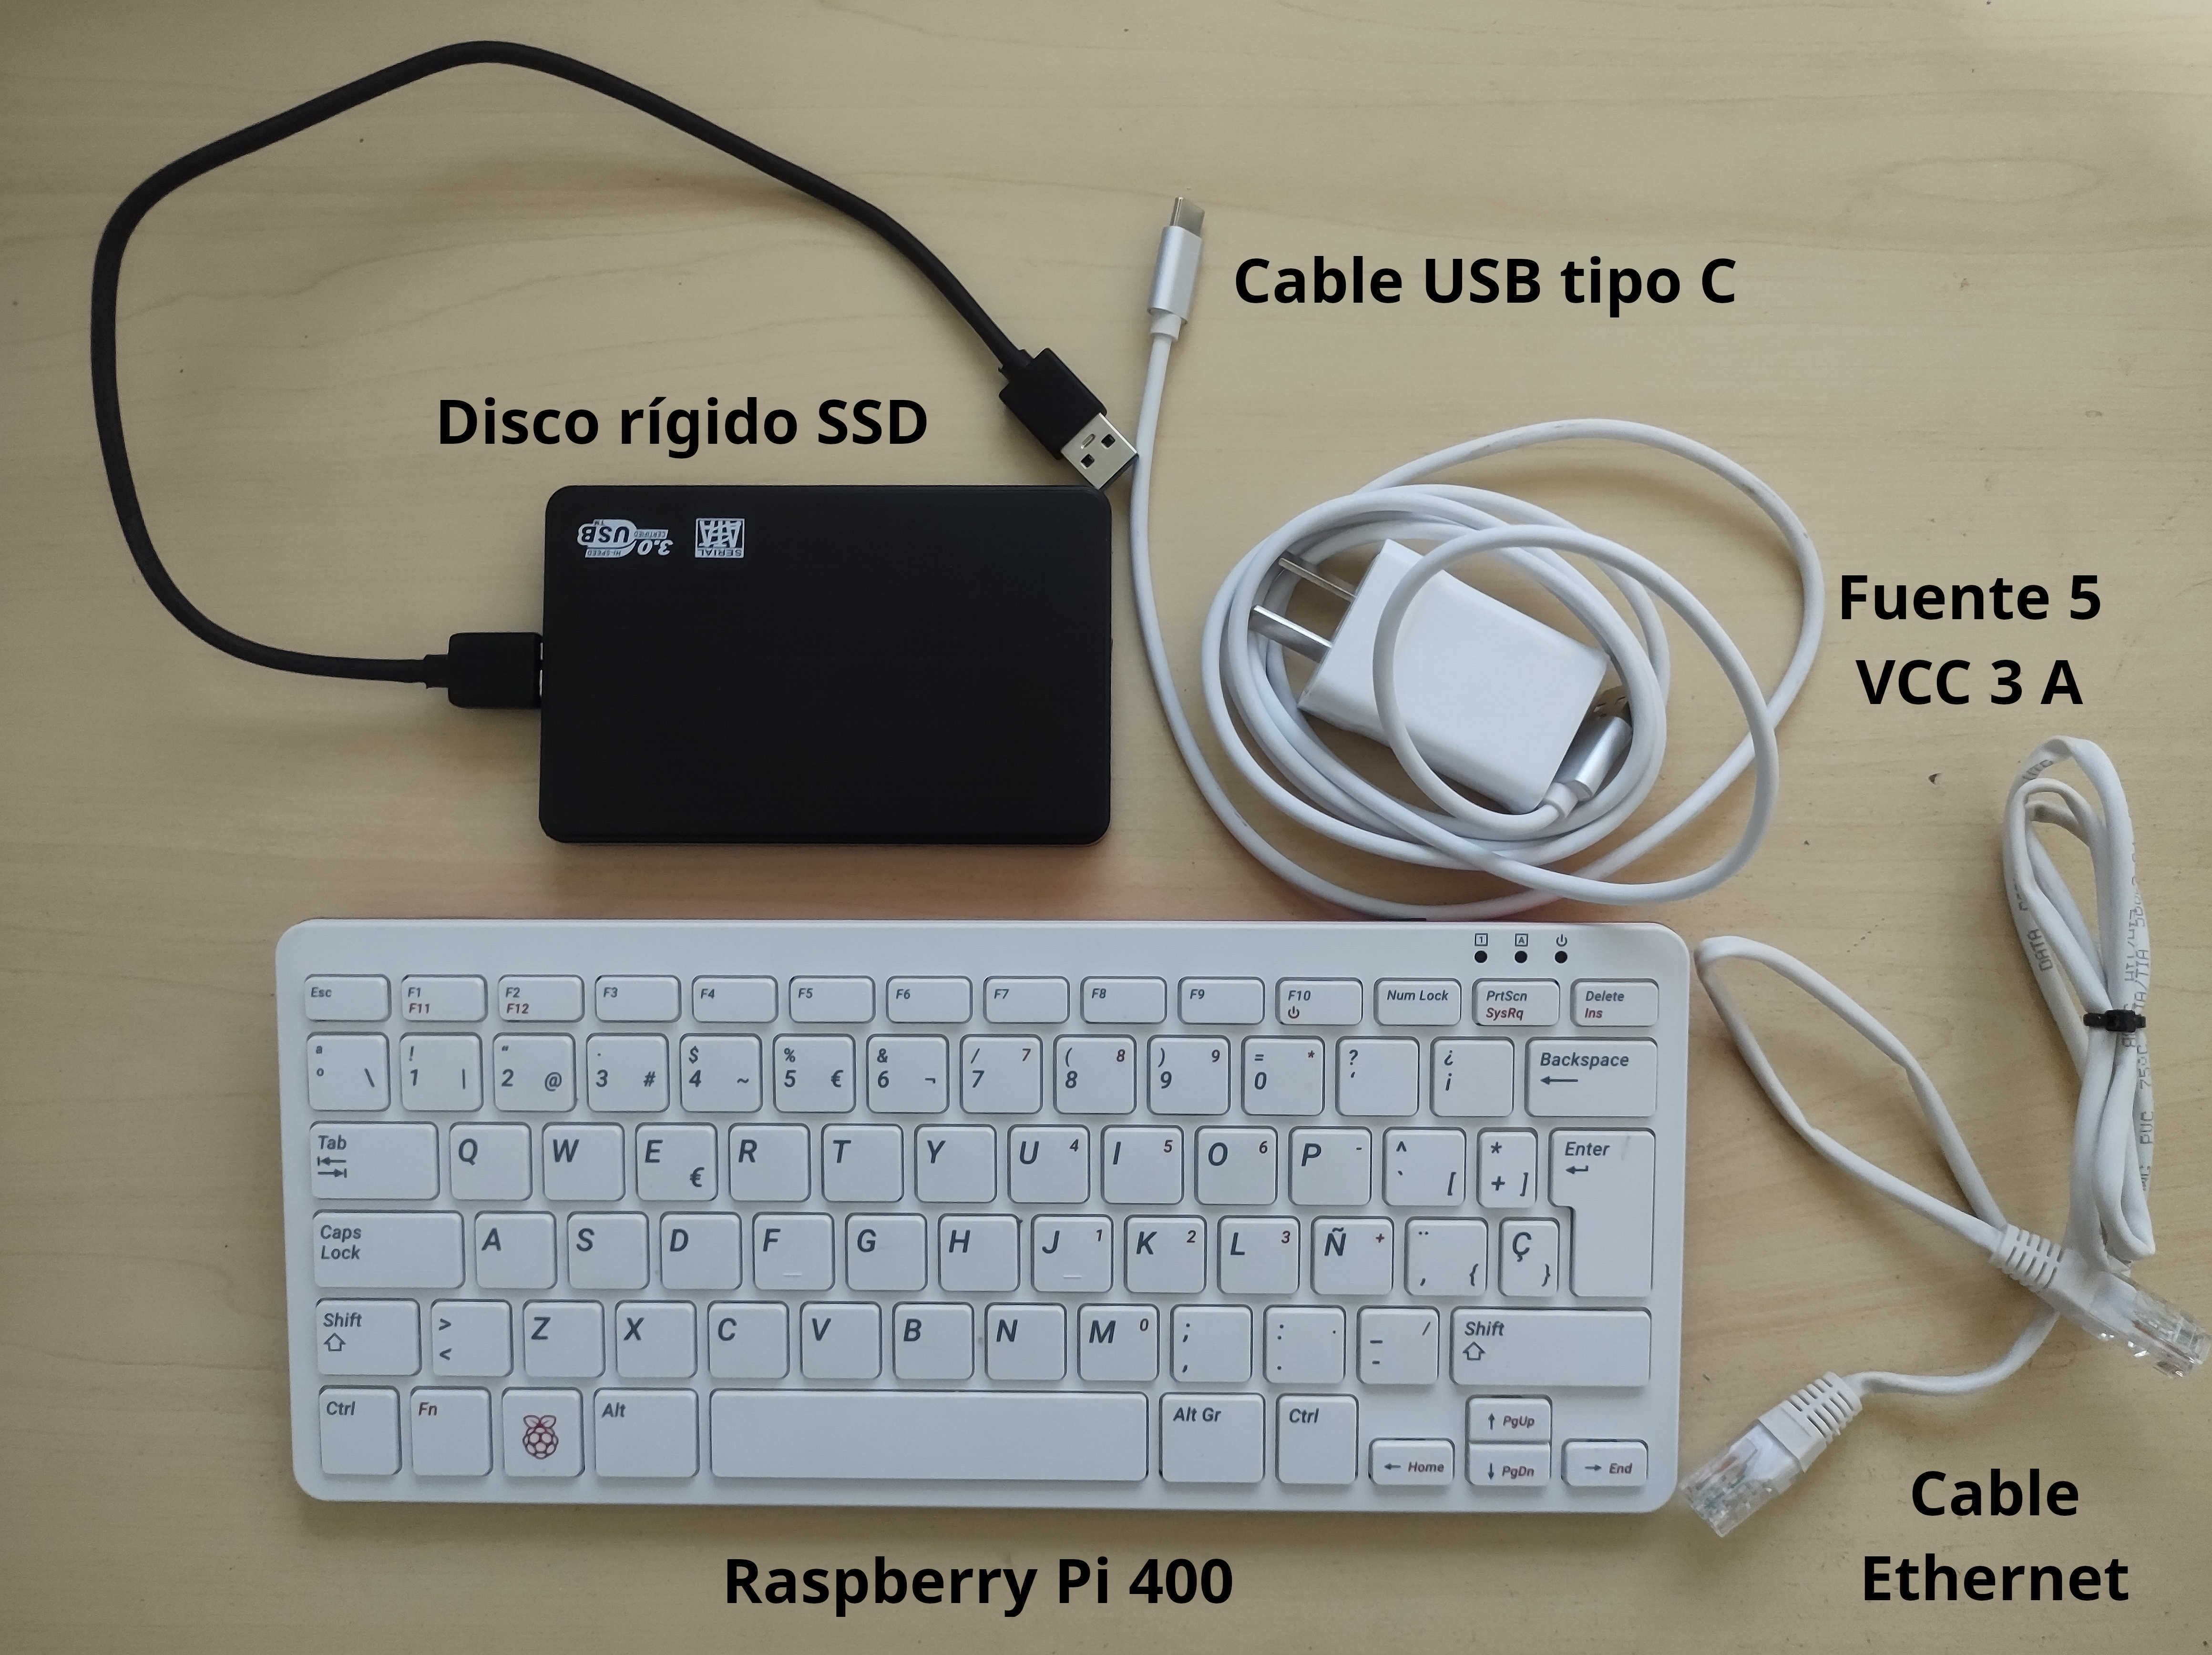
\includegraphics[scale=0.25]{Figura 33 - Servidor.jpg}
\caption[Componentes del servidor]{Componentes del servidor.}
\label{fig:33}
\end{figure}

Puede observarse la Raspberry Pi400, la fuente de 5 VCC 3 A con su cable, un disco rígido externo SSD de 120 GB y un cable Ethernet para la conexión a la red.

\section{Metodología empleada}

El hardware se testeó de forma funcional. En cuanto al software se utilizaron distintas metodologías para la depuración de forma manual de los embebidos, el frontend y el backend. A continuación, se describen cada una de ellas.

\subsection{Pruebas del frontend}

Para el frontend se utilizaron pruebas funcionales manuales con el sistema funcionando. El desarrollo fue progresivo y se llevó a cabo en paralelo. Se creó una aplicación básica y, posteriormente, se fueron agregando nuevas funcionalidades. A medida que el sistema fue creciendo, se fueron agregando más componentes hasta tener la versión actual.

En lo que respecta a las pruebas, se empleó la salida de la consola del navegador a medida que se implementaban nuevas funciones y páginas. Esto permitió exhibir en tiempo real el funcionamiento del sistema en cada página y con cada función agregada. En el código \ref{lst:console front} se muestra a modo de ejemplo parte del desarrollo de la página para la visualización de un mensaje por consola de la configuración de un dispositivo.

\begin{lstlisting}[caption={Muestra por consola de los datos recibidos.}, label={lst:console front}]
ngOnInit() {
    const deviceId = this.activatedRoute.snapshot.paramMap.get('id') as string;
    this.dispositivoId = deviceId, 10;
    this.subscription = this.dispositivoService.getDeviceById(this.dispositivoId).
   		subscribe((data) => {
      console.log(data);
      this.device = data[0];
      this.tipo = data[0].tipo;
      this.ubicacion = data[0].ubicacion;
    });
    this.leerdatos();
  }
\end{lstlisting}

Allí se puede ver la función \textit{console.log} mostrando los datos por consola. En la figura \ref{fig:34} se puede ver la pantalla de configuración del dispositivo y el mensaje por consola con los datos recibidos.

\newpage
\begin{figure}[h]
\centering
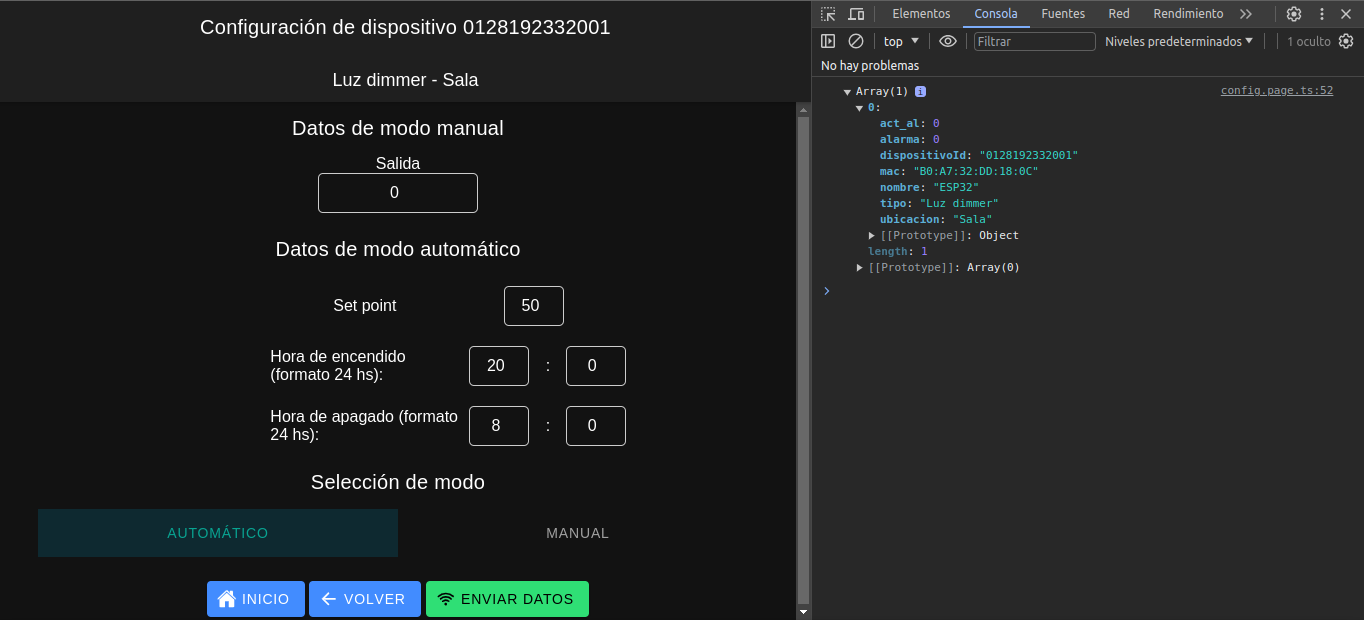
\includegraphics[scale=0.37]{Figura 34 - Consola front.png}
\caption[Pantalla de aplicación y consola del frontend]{Pantalla de aplicación y consola.}
\label{fig:34}
\end{figure}

Este mecanismo se utilizó en todas las páginas de la aplicación web y gracias a esto se consiguieron los resultados esperados de funcionalidad y depuración de errores.

\subsection{Pruebas del backend}

Para el backend se utilizó un mecanismo similar de pruebas funcionales que para el frontend.

El desarrollo siguió un enfoque progresivo lo que significa que a medida que se fueron incorporando funciones o endpoints nuevos, se fueron colocando muestras por consola para poder observar si los datos y las consultas estaban siendo resueltos de forma correcta. En el código \ref{lst:console back} se muestra como ejemplo el \textit{router} para borrar la tabla de mediciones de un dispositivo y el mensaje por consola de éxito y el ID del dispositivo.

\begin{lstlisting}[caption={Muestra por consola de los datos consultados.}, label={lst:console back}]
borrarTablaRouter.delete('/:id', async function (req, res, next) {
  const id = req.params.id;
  let connection;
  try {
      connection = await pool.getConnection();
      await connection.beginTransaction();
      const deleteMedicionesQuery = 'DELETE FROM Mediciones WHERE dispositivoId = ?';
      await connection.query(deleteMedicionesQuery, id);
      await connection.commit();
      connection.release();
      res.send({ message: 'Mediciones eliminadas exitosamente' }).status(200);
      console.log('Solicitud de eliminacion recibida para dispositivoId:', id);
      } catch (err) {
          if (connection) {
              await connection.rollback();
              connection.release();
          }
          res.send(err).status(400);
          console.log('Error al eliminar mediciones:', err);
      }
  });
\end{lstlisting}

En la figura \ref{fig:35} se puede ver la consola con el mensaje de éxito y el ID del dispositivo cuya tabla de mediciones fue eliminada.

\begin{figure}[h]
\centering
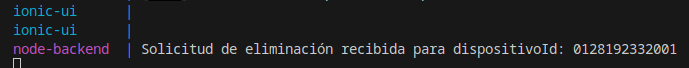
\includegraphics[scale=0.65]{Figura 35 - Consola back.png}
\caption[Mensaje por consola del servidor en el backend]{Mensaje por consola del servidor.}
\label{fig:35}
\end{figure}

Además de estas pruebas, se incorporó el uso de la aplicación \textit{MQTTX} para testear la comunicación con el \textit{broker} y los dispositivos, especialmente durante la implementación de la seguridad con los certificados SSL. De esta forma, se llevaron a cabo pruebas que abarcaron desde la primera conexión segura hasta la inserción de datos desde un dispositivo simulado, el envío de configuración desde la aplicación a los nodos y el mensaje de solicitud de configuración inicial de un nodo, entre otros.

En la figura \ref{fig:36} puede verse la configuración de \textit{MQTTX} para el envío de datos de una medición simulada en el \textit{topic \textbackslash home\textbackslash temperatura\textbackslash data} para luego verificar la correcta inserción en la base de datos.

\begin{figure}[h]
\centering
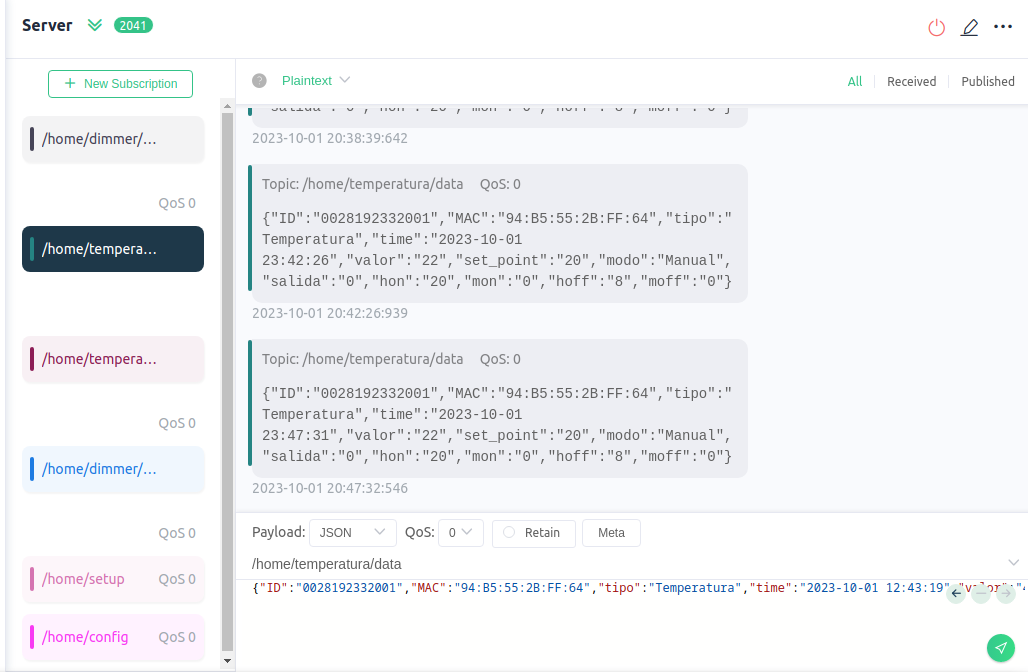
\includegraphics[scale=0.5]{Figura 36 - MQTTX.png}
\caption[Pantalla de MQTTX]{Pantalla de MQTTX.}
\label{fig:36}
\end{figure}

\subsection{Pruebas de los nodos}

El hardware se testeó haciendo pruebas de funcionamiento con los materiales mencionados en la sección anterior. Las pruebas consistieron en poner en funcionamiento los nodos durante dos días consecutivos, verificando que el control de temperatura funcionara dentro de los valores configurados y que la luminaria se encendiera y mantuviera los valores de los saltos. También se evaluó el funcionamiento de los horarios de encendido y apagado.

En cuanto al software, las placas ESP32 poseen comunicación serial incorporada por lo que se colocaron funciones de muestra por consola al momento de incorporar funcionalidades nuevas. En el código \ref{lst:dispositivo}, se puede ver un ejemplo de cómo se utilizó la función \textit{ESP\_LOGI} para mostrar por consola el valor de la salida recibido por MQTT.

\lstset{frame=tb,
  language=C++,
  aboveskip=3mm,
  belowskip=3mm,
  captionpos=b,
  showstringspaces=false,
  columns=flexible,
  basicstyle={\small\ttfamily},
  numbers=left,
  numberstyle=\tiny\color{gray},
  keywordstyle=\color{blue},
  commentstyle=\color{dkgreen},
  stringstyle=\color{mauve},
  breaklines=true,
  breakatwhitespace=true,
  tabsize=3,
}

\begin{lstlisting}[caption={Muestra por consola de la terminal ESP-IDF.}, label={lst:dispositivo}]
const cJSON *salida = cJSON_GetObjectItemCaseSensitive(root, "salida");
    if (cJSON_IsNumber(salida) && select) {
        if(salida->valueint==100)
            out_temp=true;
        if(salida->valueint==0)
            out_temp=false;
        ESP_LOGI(TAG, "Received MQTT salida: %d", salida->valueint);
        pant_main();
    }
\end{lstlisting}

En este caso se muestra por consola el mensaje de recepción del valor de salida y su valor correspondiente.

\section{Resultados finales}

Para la prueba final, se ensamblaron los 2 nodos, y se conectó un calefactor eléctrico de 750 W al nodo de temperatura. En el lado del servidor, se ejecutó el \textit{docker-compose} con el sistema completo. Se realizaron ajustes tanto desde la aplicación web como de cada uno de los nodos.

En la figura \ref{fig:37}, se puede observar el nodo de iluminación funcionando encendido, y en la pantalla se muestra el valor de la salida.

\begin{figure}[h]
\centering
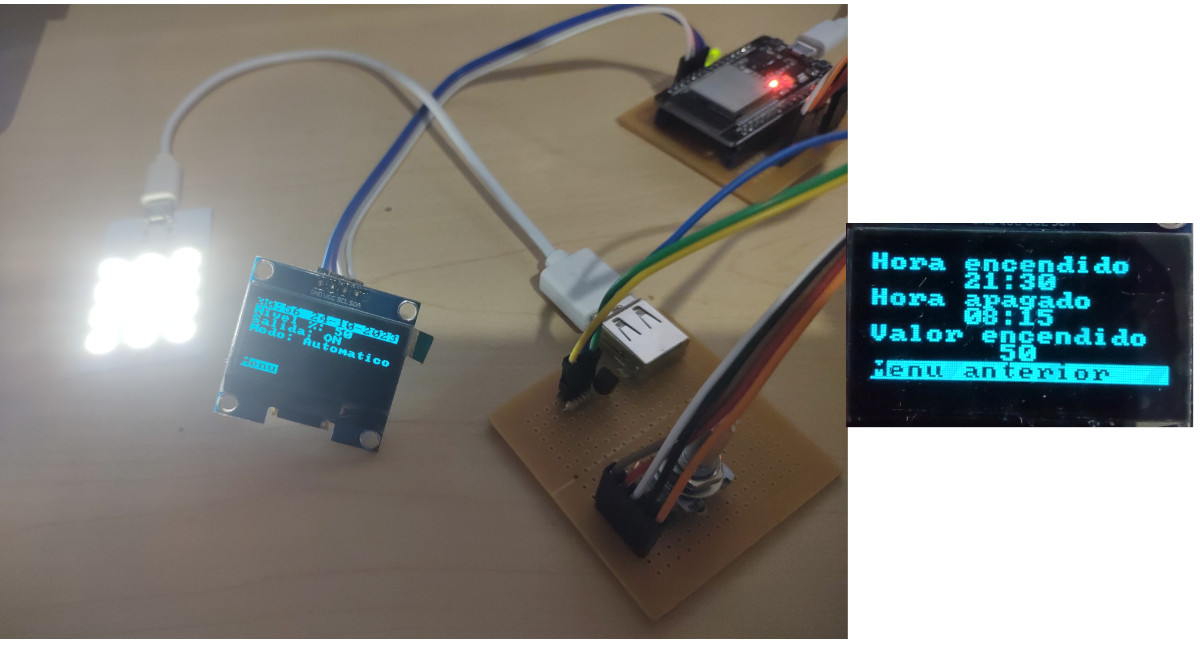
\includegraphics[scale=0.06]{Figura 37 - Dimmer funcionando.jpg}
\caption[Dimmer en modo automático funcionando]{Dimmer en modo automático funcionando.}
\label{fig:37}
\end{figure}

En la figura \ref{fig:38}, se puede observar la pantalla de configuración de modo automático.

\begin{figure}[h]
\centering
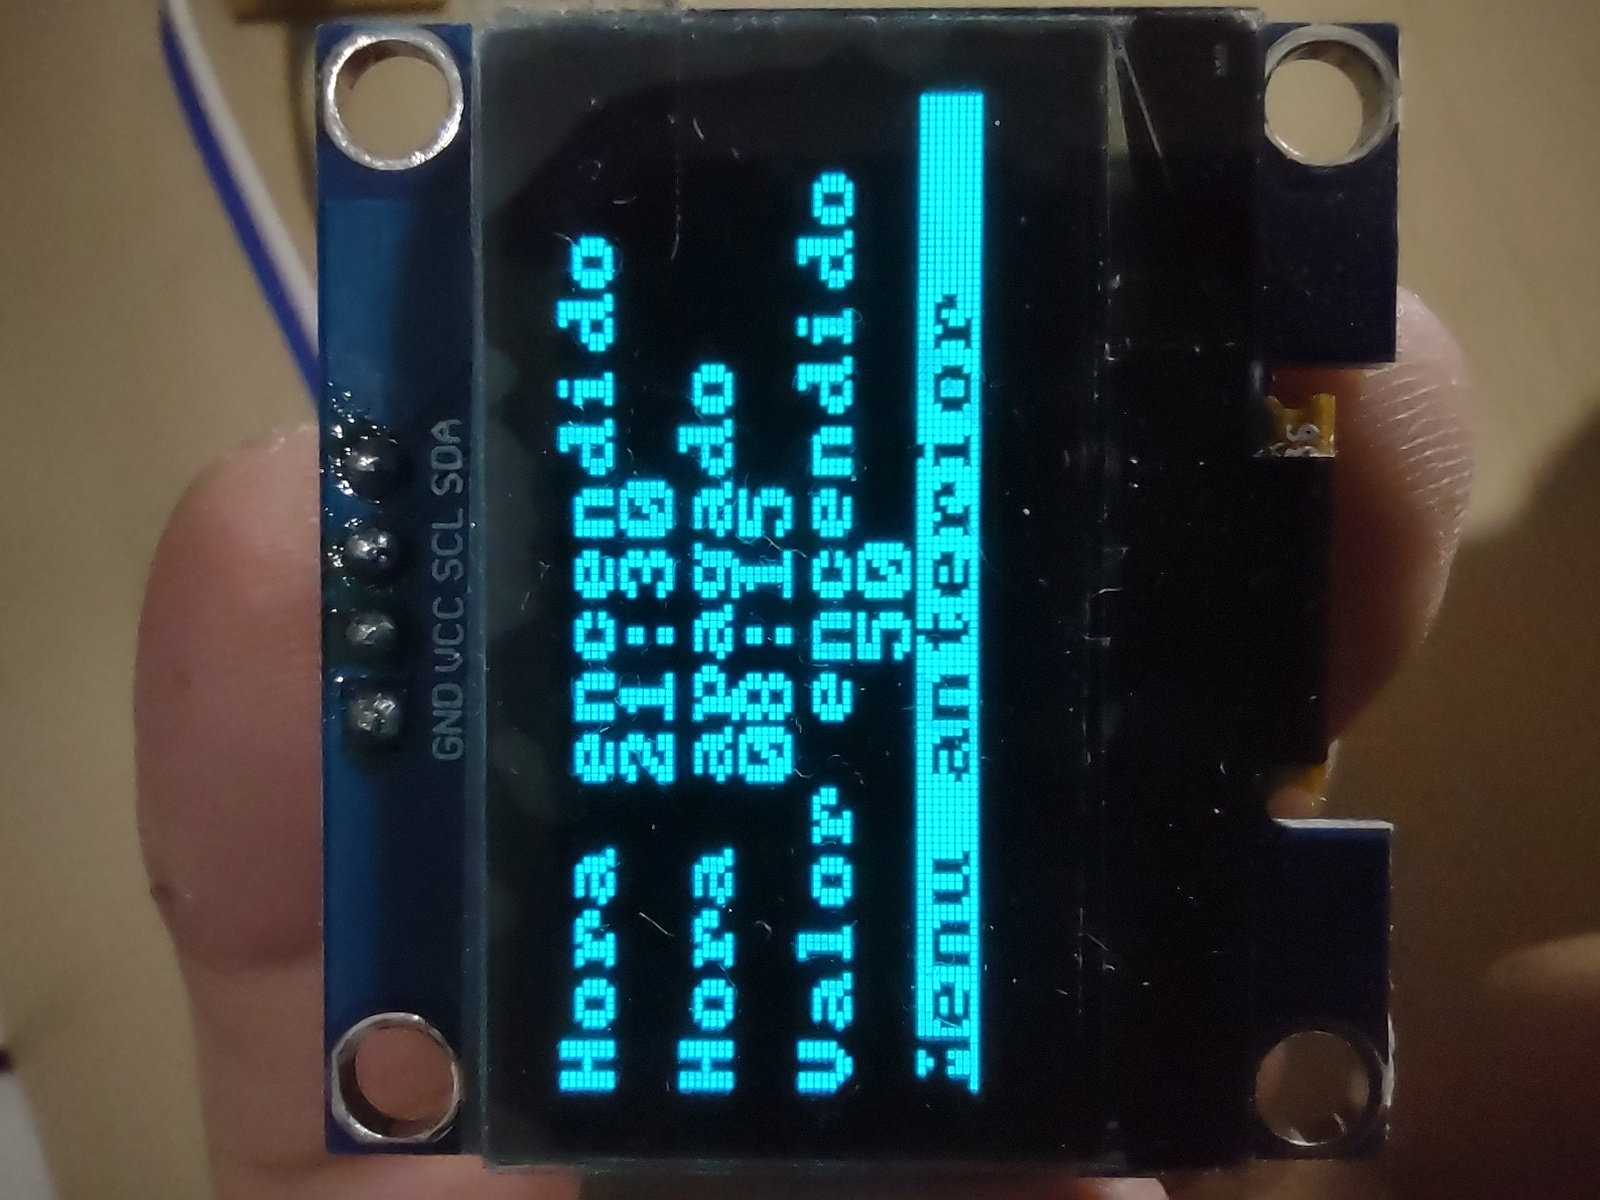
\includegraphics[angle=270, scale=0.47]{Figura 38 - Pantalla dimmer funcionando.jpg}
\caption[Pantalla de configuración del dimmer en modo automático]{Pantalla de configuración del dimmer en modo automático.}
\label{fig:38}
\end{figure}

En la figura \ref{fig:39} puede observarse la página de configuración del nodo dimmer. Puede observarse que los datos ingresados corresponden con los datos guardados en el nodo, y que este último está funcionando según lo esperado.

\begin{figure}[h]
\centering
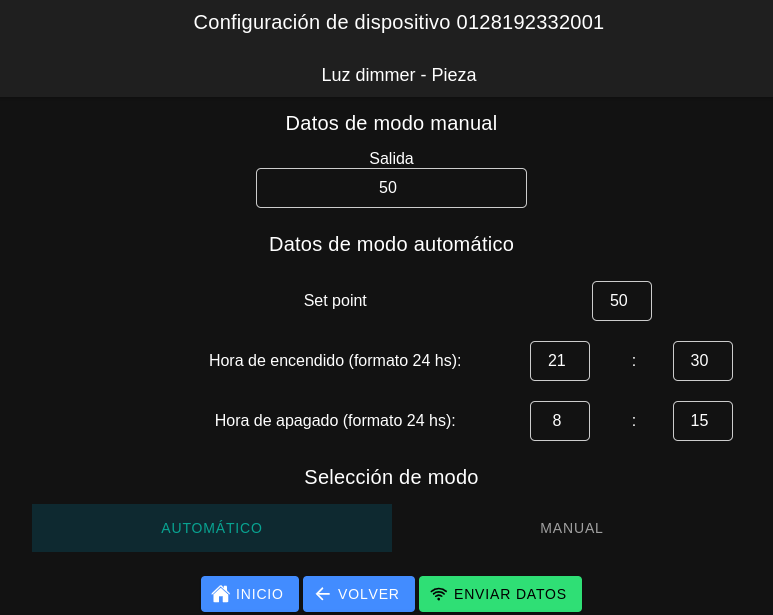
\includegraphics[scale=0.45]{Figura 39 - Config.png}
\caption[Pantalla de configuración de dimmer]{Pantalla de configuración de dimmer.}
\label{fig:39}
\end{figure}

Se ha verificado la capacidad de agregar y modificar los datos de los dispositivos desde la página correspondiente, contrastando los datos visualizados en la pantalla de \textit{phpMyAdmin}. Durante una prueba que se realizó, se cargó un dispositivo nuevo y se corroboró tanto desde la aplicación del sistema como desde la página de administración de la base de datos. En la figura \ref{fig:40} puede verse cómo se agregó un dispositivo nuevo desde la página en la parte superior y cómo se ve reflejado en la base de datos en la inferior.

\newpage
\begin{figure}[h]
\centering
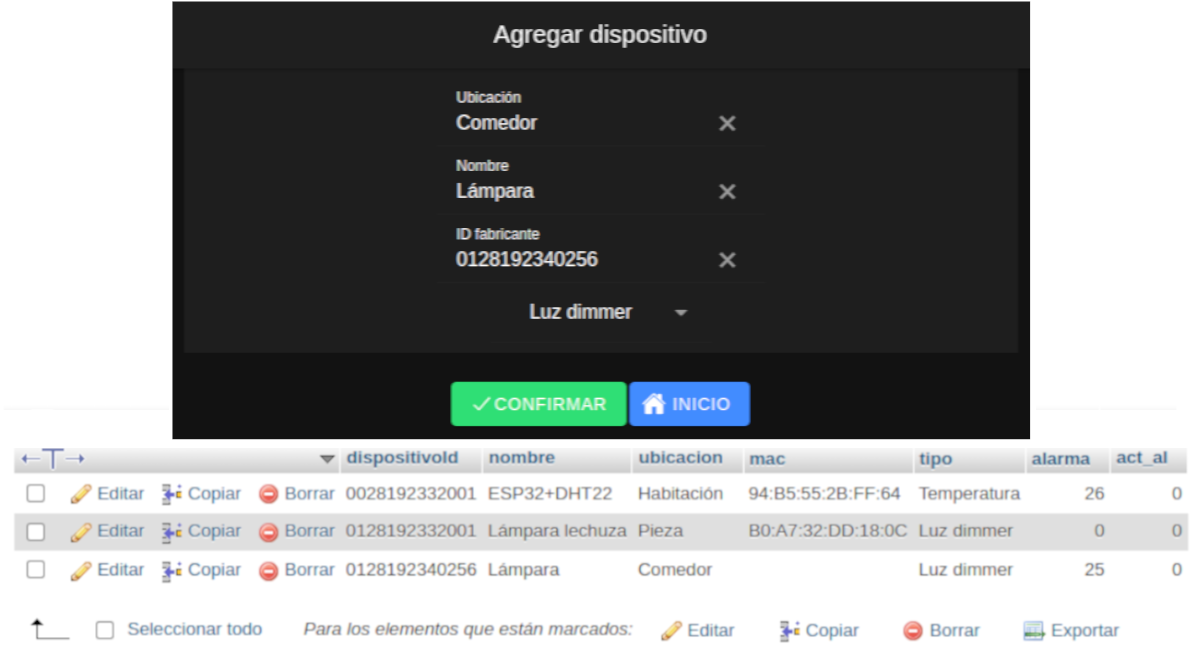
\includegraphics[scale=0.33]{Figura 40 - Agregar dispositivo.png}
\caption[Valores de dispositivo nuevo al agregar dispositivo]{Valores de dispositivo nuevo.}
\label{fig:40}
\end{figure}

Aquí se observa que los datos cargados coinciden con los almacenados. La diferencia radica en que no se registró la MAC del dispositivo ya que al momento de obtener la imagen el dispositivo no había emitido datos al servidor.

Algo similar a la prueba de los dispositivos se hizo con los usuarios. El sistema por default tiene los valores \textit{user1}, \textit{user2} y \textit{user3} y contraseña \textit{user}. Esto se logró creando estos usuarios con sus datos en el archivo de creación de la base de datos \textit{domotica.sql}. En la figura \ref{fig:41} se muestran los valores ingresados en la página de configuración en la parte superior y los que están almacenados en la base de datos en la inferior. Como se puede observar en la imagen, los valores cargados desde la página coinciden con los almacenados en la base de datos.

\begin{figure}[h]
\centering
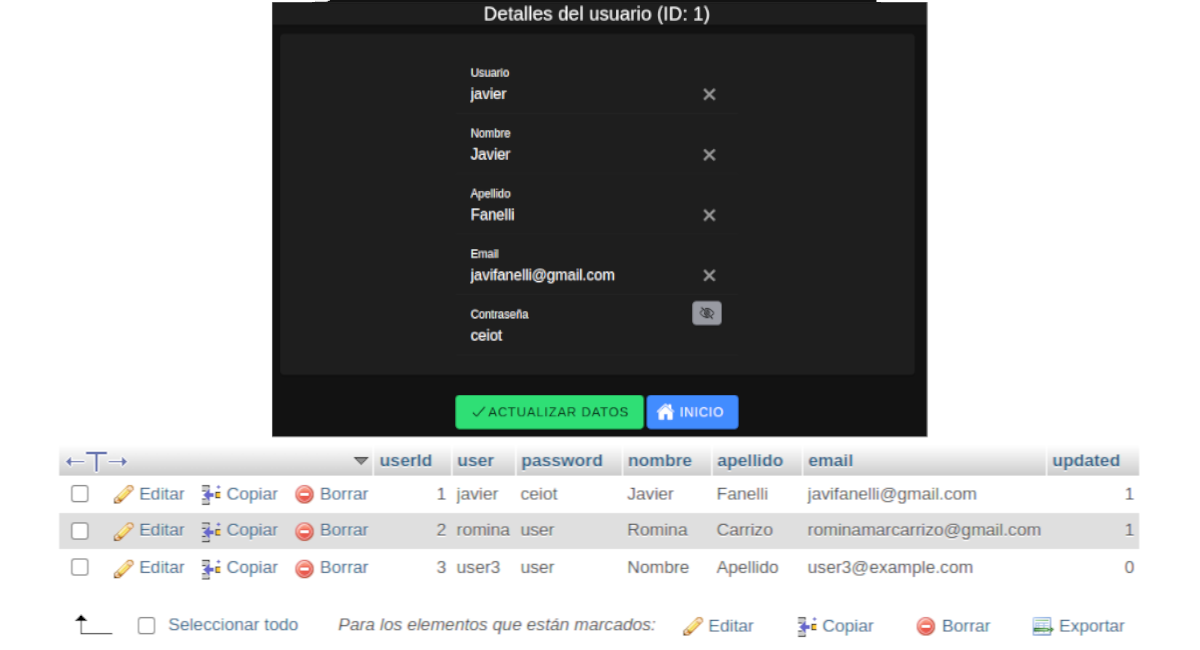
\includegraphics[scale=0.34]{Figura 41 - Modificar usuario.png}
\caption[Valores de usuario modificados]{Valores de usuario modificados.}
\label{fig:41}
\end{figure}

Por último, se hizo la corroboración de la activación de la alarma y el envío del mail. En la figura \ref{fig:42} puede observarse la configuración del dispositivo en la parte superior y el mail recibido en la parte inferior.

\begin{figure}[h]
\centering
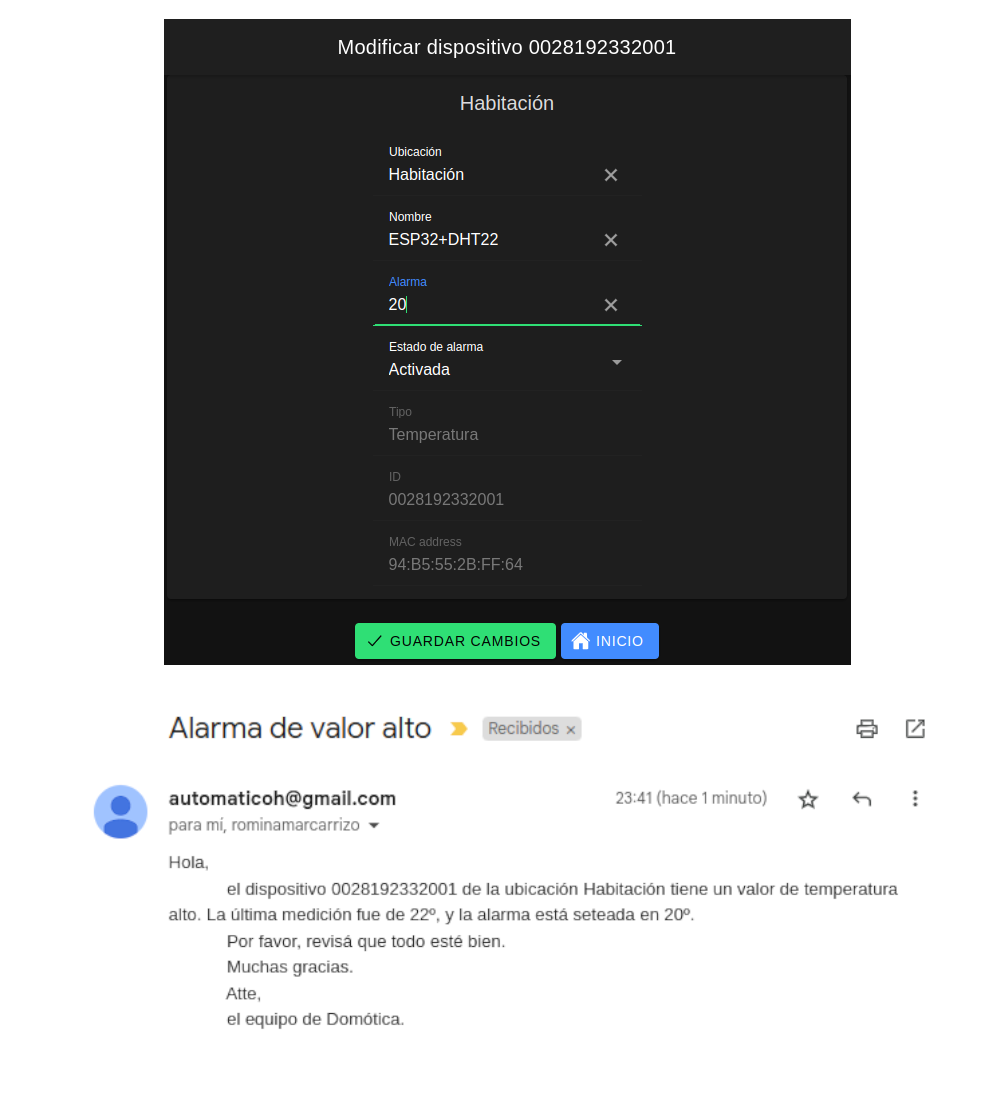
\includegraphics[scale=0.35]{Figura 42 - Alarma.png}
\caption[Envío de alarma de medición]{Envío de alarma de medición.}
\label{fig:42}
\end{figure}

De este modo, se realizaron las pruebas más importantes de funcionalidades del sistema. Al dar resultados de funcionamiento satisfactorios, se concluye que la aplicación funciona de manera correcta.

\section{Comparación con el estado del arte}

En la tabla \ref{tab:estadoarte} se encuentra la comparación entre las soluciones de hogares inteligentes existentes en el mercado nacional, Domotic y Reactor, y el trabajo realizado. 

\newpage
\begin{table}[h]
\centering
\caption[Comparativa entre las distintas opciones - Estado del arte]{Comparativa entre las distintas opciones.}
\begin{tabular}{l c c c}
\toprule
\textbf{Funcionalidad} & \textbf{Domotic} & \textbf{Reactor} & \textbf{Trabajo final}\\
\midrule
Posee unidad central			& Sí		& No		& Sí\\
Capacidad de diseño de		&		&		&\\
dispositivos nuevos			& Sí		& Sí		& Sí\\
Almacenamiento de mediciones	& No		& Sí		& Sí\\
Programación de reacciones	& Sí		& Sí		& Sí\\
Aplicación en ambientes		&		&		&\\
profesionales y oficinas		& No		& Sí		& Sí\\
Avisos por mail				& No		& Sí		& Sí\\
Aplicación móvil				& Sí		& Sí		& No\\
Conexión	 desde el exterior	& Sí		& Sí		& No\\
\bottomrule
\hline
\end{tabular}
\label{tab:estadoarte}
\end{table}

Como se puede observar de la tabla comparativa, el trabajo está a la par de otras soluciones similares. Entre sus puntos positivos, el sistema desarrollado posee una unidad central, en este caso, el servidor, que puede aceptar diseños nuevos de dispositivos, proporciona notificaciones en caso de eventos y almacena valores de mediciones que sean útiles.

En cuanto a los aspectos a mejorar se describirán en el capítulo 5 en la sección de trabajo futuro. 
\chapter{Conclusiones}

\label{Chapter5}

En el presente capítulo se detallan los resultados obtenidos del trabajo realizado y se describen las mejoras en un posible trabajo futuro.

\section{Resultados obtenidos}

En este trabajo se concluyó el desarrollo y pruebas funcionales de un prototipo de sistema de automatización de hogares, contando con 2 tipos de dispositivos.

Para evaluar los resultados finales, es necesario analizar los siguientes temas:

\begin{itemize}
	\item Se cumplió con las fechas finales de finalización del trabajo, aunque la realización de las tareas en la práctica difirió un poco de lo planificado. Se planificaron las tareas de forma muy secuencial pero se hicieron algunas de ellas en paralelo junto con otras.
	\item No se manifestó ninguno de los riesgos advertidos en la planificación, aunque se siguieron todas las medidas de mitigación de aquellos riesgos más graves.
	\item Se lograron cumplir con todos los requerimientos presentados y pactados con el cliente. Aunque hubo una modificación que llevó a desglosar al nodo previsto que cubra todas las funciones con dos nodos que tengan funciones específicas.
\end{itemize}

Fueron de gran aporte y utilidad todos los conocimientos adquiridos en el transcurso del posgrado, y en especial aquellos conocimientos adquiridos en las materias que se listan a continuación:

\begin{itemize}
	\item Protocolos de internet.
	\item Arquitecturas de datos.
	\item Arquitecturas de protocolos.
	\item Desarrollo de aplicaciones multiplataforma.
	\item Desarrollo de aplicaciones para internet de las cosas.
\end{itemize}

\section{Trabajo futuro}

A continuación se describen aquellas tareas para lograr mejoras en el sistema cuya continuación será en un posible trabajo futuro:

\begin{itemize}
	\item Hacer aplicaciones móviles para Android y IOS, ya que el desarrollo fue hecho en Ionic con este propósito.
	\item Implementar un \textit{access point} en el servidor para que los dispositivos se conecten automáticamente a él una vez que sean encendidos por primera vez.
	\item Implementar actualizaciones de software OTA en los dispositivos.
	\item Integración con sistemas de seguridad y cámaras.
	\item Mejoras en la interfaz gráfica de la web tales como el uso de menúes en las páginas en lugar de usar solo botones.
	\item Integración con Google Assistant.
	\item Implementación de un servicio en la nube para el acceso fuera del hogar o edificación, manteniendo todas las otras funcionalidades en el servidor local.
	\item Implementación de niveles de usuarios para que haya un usuario \textit{root} que pueda crear cuantos usuarios desee y los administre.
	\item Implementación de alarmas y avisos a través de la aplicación móvil o web y a través de plataformas como Telegram.
\end{itemize} 

%----------------------------------------------------------------------------------------
%	CONTENIDO DE LA MEMORIA  - APÉNDICES
%----------------------------------------------------------------------------------------

\appendix % indicativo para indicarle a LaTeX los siguientes "capítulos" son apéndices

% Incluir los apéndices de la memoria como archivos separadas desde la carpeta Appendices
% Descomentar las líneas a medida que se escriben los apéndices

% Appendix A

\chapter{Ejemplo de creación de menú en ESP32} % Main appendix title

En este anexo se describe un ejemplo de manejo del menú principal en los nodos.

\label{AppendixA} % For referencing this appendix elsewhere, use \ref{AppendixA}

\begin{lstlisting}[caption={Código del menú principal.}, label={lst:Ejemplo menu}]
void menu1 (void)
{
	ssd1306_clear_screen(&devd, false);
	pos_menu=1;
	while(level==1){
		if(inc_enc){
			pos_menu++;
			inc_enc=false;
			if (pos_menu>6)
				pos_menu=1;
		}	
		if (dec_enc){
			pos_menu--;
			dec_enc=false;
			if (pos_menu<1)
				pos_menu=6;
		}
		if(pos_menu==1){
			ssd1306_display_text(&devd, 0, "Estado          ", 16, true);
			ssd1306_display_text(&devd, 1, "Info conexion   ", 16, false);
			ssd1306_display_text(&devd, 2, "Modo            ", 16, false);
			ssd1306_display_text(&devd, 3, "Conf modo auto  ", 16, false);
			ssd1306_display_text(&devd, 4, "Actualizar hora ", 16, false);
			ssd1306_display_text(&devd, 5, "Pant. principal ", 16, false);
			if(btn_enc){
				btn_enc=false;
				level=10;
			}
		}
		if(pos_menu==2){
			ssd1306_display_text(&devd, 0, "Estado          ", 16, false);
			ssd1306_display_text(&devd, 1, "Info conexion   ", 16, true);
			ssd1306_display_text(&devd, 2, "Modo            ", 16, false);
			ssd1306_display_text(&devd, 3, "Conf modo auto  ", 16, false);
			ssd1306_display_text(&devd, 4, "Actualizar hora ", 16, false);
			ssd1306_display_text(&devd, 5, "Pant. principal ", 16, false);
			if(btn_enc){
				btn_enc=false;
				level=11;
			}
		}
		if(pos_menu==3){
			ssd1306_display_text(&devd, 0, "Estado          ", 16, false);
			ssd1306_display_text(&devd, 1, "Info conexion   ", 16, false);
			ssd1306_display_text(&devd, 2, "Modo            ", 16, true);
			ssd1306_display_text(&devd, 3, "Conf modo auto  ", 16, false);
			ssd1306_display_text(&devd, 4, "Actualizar hora ", 16, false);
			ssd1306_display_text(&devd, 5, "Pant. principal ", 16, false);	
			if(btn_enc){
				btn_enc=false;
				level=2;
			}
		}
		if(pos_menu==4){
			ssd1306_display_text(&devd, 0, "Estado          ", 16, false);
			ssd1306_display_text(&devd, 1, "Info conexion   ", 16, false);
			ssd1306_display_text(&devd, 2, "Modo            ", 16, false);
			ssd1306_display_text(&devd, 3, "Conf modo auto  ", 16, true);
			ssd1306_display_text(&devd, 4, "Actualizar hora ", 16, false);
			ssd1306_display_text(&devd, 5, "Pant. principal ", 16, false);	
			if(btn_enc){
				btn_enc=false;
				level=3;
			}
		}
		if(pos_menu==5){
			ssd1306_display_text(&devd, 0, "Estado          ", 16, false);
			ssd1306_display_text(&devd, 1, "Info conexion   ", 16, false);
			ssd1306_display_text(&devd, 2, "Modo            ", 16, false);
			ssd1306_display_text(&devd, 3, "Conf modo auto  ", 16, false);
			ssd1306_display_text(&devd, 4, "Actualizar hora ", 16, true);
			ssd1306_display_text(&devd, 5, "Pant. principal ", 16, false);
			if(btn_enc){
				btn_enc=false;
				ssd1306_display_text(&devd, 6, "Obteniendo la", 13, false);
    			ssd1306_display_text(&devd, 7, "hora...", 7, false);
				obtain_time();
				ssd1306_display_text(&devd, 7, "hora... OK", 10, false);
				vTaskDelay(pdMS_TO_TICKS(1000));
				ssd1306_display_text(&devd, 6, "               ", 15, false);
				ssd1306_display_text(&devd, 7, "               ", 15, false);
			}
		}
		if(pos_menu==6){
			ssd1306_display_text(&devd, 0, "Estado          ", 16, false);
			ssd1306_display_text(&devd, 1, "Info conexion   ", 16, false);
			ssd1306_display_text(&devd, 2, "Modo            ", 16, false);
			ssd1306_display_text(&devd, 3, "Conf modo auto  ", 16, false);
			ssd1306_display_text(&devd, 4, "Actualizar hora ", 16, false);
			ssd1306_display_text(&devd, 5, "Pant. principal ", 16, true);
			if (btn_enc){
				btn_enc=false;
				level=0;	
			}
		}
	}
	if(level==10){
			if (net_con)
				pant_conok();
			if (!net_con)
				pant_nocon();
	}
	if(level==11){
		pant_est();
	}
	if(level==2){
		menu2();
	}
	if(level==3){
		menu3();
	}
	if(level==0){
		pant_main();
	}
}
\end{lstlisting}
%\include{Appendices/AppendixB}
%\include{Appendices/AppendixC}

%----------------------------------------------------------------------------------------
%	BIBLIOGRAPHY
%----------------------------------------------------------------------------------------

\Urlmuskip=0mu plus 1mu\relax
\raggedright
\printbibliography[heading=bibintoc]

%----------------------------------------------------------------------------------------

\end{document}  
